% This file was created with tikzplotlib v0.10.1.
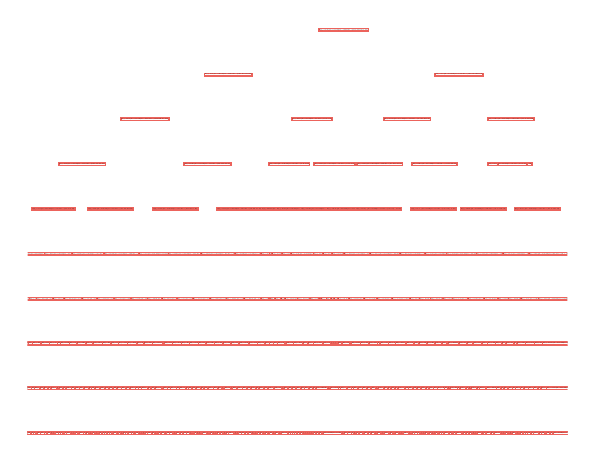
\begin{tikzpicture}

\definecolor{darkgray176}{RGB}{176,176,176}
\definecolor{tomato2369992}{RGB}{236,99,92}

\begin{axis}[
hide x axis,
hide y axis,
tick align=outside,
tick pos=left,
x grid style={darkgray176},
xmin=0, xmax=1,
xtick style={color=black},
y grid style={darkgray176},
ymin=0, ymax=1,
ytick style={color=black}
]
\draw (axis cs:0.00192307692307692,0.05) node[
  scale=0.05,
  fill=white,
  draw=tomato2369992,
  line width=0.6pt,
  inner sep=3.6pt,
  text=black,
  rotate=0.0,
  align=center
]{gini = 0.038
samples = 3572
value = [3503, 3, 0, 66]};
\draw (axis cs:0.00576923076923077,0.05) node[
  scale=0.05,
  fill=white,
  draw=tomato2369992,
  line width=0.6pt,
  inner sep=3.6pt,
  text=black,
  rotate=0.0,
  align=center
]{gini = 0.109
samples = 245
value = [231, 11, 0, 3]};
\draw (axis cs:0.00961538461538462,0.05) node[
  scale=0.05,
  fill=white,
  draw=tomato2369992,
  line width=0.6pt,
  inner sep=3.6pt,
  text=black,
  rotate=0.0,
  align=center
]{gini = 0.077
samples = 903
value = [867, 0, 0, 36]};
\draw (axis cs:0.0134615384615385,0.05) node[
  scale=0.05,
  fill=white,
  draw=tomato2369992,
  line width=0.6pt,
  inner sep=3.6pt,
  text=black,
  rotate=0.0,
  align=center
]{gini = 0.401
samples = 18
value = [13, 0, 0, 5]};
\draw (axis cs:0.0173076923076923,0.05) node[
  scale=0.05,
  fill=white,
  draw=tomato2369992,
  line width=0.6pt,
  inner sep=3.6pt,
  text=black,
  rotate=0.0,
  align=center
]{gini = 0.32
samples = 5
value = [1, 0, 0, 4]};
\draw (axis cs:0.0211538461538462,0.05) node[
  scale=0.05,
  fill=white,
  draw=tomato2369992,
  line width=0.6pt,
  inner sep=3.6pt,
  text=black,
  rotate=0.0,
  align=center
]{gini = 0.245
samples = 7
value = [6, 1, 0, 0]};
\draw (axis cs:0.025,0.05) node[
  scale=0.05,
  fill=white,
  draw=tomato2369992,
  line width=0.6pt,
  inner sep=3.6pt,
  text=black,
  rotate=0.0,
  align=center
]{gini = 0.0
samples = 1
value = [0, 0, 0, 1]};
\draw (axis cs:0.0288461538461538,0.05) node[
  scale=0.05,
  fill=white,
  draw=tomato2369992,
  line width=0.6pt,
  inner sep=3.6pt,
  text=black,
  rotate=0.0,
  align=center
]{gini = 0.125
samples = 239
value = [223, 0, 0, 16]};
\draw (axis cs:0.0326923076923077,0.05) node[
  scale=0.05,
  fill=white,
  draw=tomato2369992,
  line width=0.6pt,
  inner sep=3.6pt,
  text=black,
  rotate=0.0,
  align=center
]{gini = 0.463
samples = 11
value = [7, 0, 0, 4]};
\draw (axis cs:0.0365384615384615,0.05) node[
  scale=0.05,
  fill=white,
  draw=tomato2369992,
  line width=0.6pt,
  inner sep=3.6pt,
  text=black,
  rotate=0.0,
  align=center
]{gini = 0.198
samples = 9
value = [8, 0, 0, 1]};
\draw (axis cs:0.0403846153846154,0.05) node[
  scale=0.05,
  fill=white,
  draw=tomato2369992,
  line width=0.6pt,
  inner sep=3.6pt,
  text=black,
  rotate=0.0,
  align=center
]{gini = 0.0
samples = 2
value = [0, 2, 0, 0]};
\draw (axis cs:0.0442307692307692,0.05) node[
  scale=0.05,
  fill=white,
  draw=tomato2369992,
  line width=0.6pt,
  inner sep=3.6pt,
  text=black,
  rotate=0.0,
  align=center
]{gini = 0.461
samples = 16
value = [11, 4, 0, 1]};
\draw (axis cs:0.0480769230769231,0.05) node[
  scale=0.05,
  fill=white,
  draw=tomato2369992,
  line width=0.6pt,
  inner sep=3.6pt,
  text=black,
  rotate=0.0,
  align=center
]{gini = 0.0
samples = 1
value = [0, 1, 0, 0]};
\draw (axis cs:0.0519230769230769,0.05) node[
  scale=0.05,
  fill=white,
  draw=tomato2369992,
  line width=0.6pt,
  inner sep=3.6pt,
  text=black,
  rotate=0.0,
  align=center
]{gini = 0.222
samples = 102
value = [89, 13, 0, 0]};
\draw (axis cs:0.0557692307692308,0.05) node[
  scale=0.05,
  fill=white,
  draw=tomato2369992,
  line width=0.6pt,
  inner sep=3.6pt,
  text=black,
  rotate=0.0,
  align=center
]{gini = 0.0
samples = 1
value = [0, 1, 0, 0]};
\draw (axis cs:0.0596153846153846,0.05) node[
  scale=0.05,
  fill=white,
  draw=tomato2369992,
  line width=0.6pt,
  inner sep=3.6pt,
  text=black,
  rotate=0.0,
  align=center
]{gini = 0.0
samples = 3
value = [0, 0, 0, 3]};
\draw (axis cs:0.0634615384615385,0.05) node[
  scale=0.05,
  fill=white,
  draw=tomato2369992,
  line width=0.6pt,
  inner sep=3.6pt,
  text=black,
  rotate=0.0,
  align=center
]{gini = 0.452
samples = 36
value = [25, 9, 0, 2]};
\draw (axis cs:0.0673076923076923,0.05) node[
  scale=0.05,
  fill=white,
  draw=tomato2369992,
  line width=0.6pt,
  inner sep=3.6pt,
  text=black,
  rotate=0.0,
  align=center
]{gini = 0.0
samples = 2
value = [0, 2, 0, 0]};
\draw (axis cs:0.0711538461538462,0.05) node[
  scale=0.05,
  fill=white,
  draw=tomato2369992,
  line width=0.6pt,
  inner sep=3.6pt,
  text=black,
  rotate=0.0,
  align=center
]{gini = 0.0
samples = 3
value = [3, 0, 0, 0]};
\draw (axis cs:0.075,0.05) node[
  scale=0.05,
  fill=white,
  draw=tomato2369992,
  line width=0.6pt,
  inner sep=3.6pt,
  text=black,
  rotate=0.0,
  align=center
]{gini = 0.0
samples = 1
value = [0, 0, 0, 1]};
\draw (axis cs:0.0788461538461538,0.05) node[
  scale=0.05,
  fill=white,
  draw=tomato2369992,
  line width=0.6pt,
  inner sep=3.6pt,
  text=black,
  rotate=0.0,
  align=center
]{gini = 0.147
samples = 64
value = [59, 2, 0, 3]};
\draw (axis cs:0.0826923076923077,0.05) node[
  scale=0.05,
  fill=white,
  draw=tomato2369992,
  line width=0.6pt,
  inner sep=3.6pt,
  text=black,
  rotate=0.0,
  align=center
]{gini = 0.0
samples = 60
value = [60, 0, 0, 0]};
\draw (axis cs:0.0865384615384615,0.05) node[
  scale=0.05,
  fill=white,
  draw=tomato2369992,
  line width=0.6pt,
  inner sep=3.6pt,
  text=black,
  rotate=0.0,
  align=center
]{gini = 0.18
samples = 10
value = [9, 0, 0, 1]};
\draw (axis cs:0.0903846153846154,0.05) node[
  scale=0.05,
  fill=white,
  draw=tomato2369992,
  line width=0.6pt,
  inner sep=3.6pt,
  text=black,
  rotate=0.0,
  align=center
]{gini = 0.0
samples = 1
value = [0, 0, 0, 1]};
\draw (axis cs:0.0942307692307692,0.05) node[
  scale=0.05,
  fill=white,
  draw=tomato2369992,
  line width=0.6pt,
  inner sep=3.6pt,
  text=black,
  rotate=0.0,
  align=center
]{gini = 0.32
samples = 15
value = [3, 0, 0, 12]};
\draw (axis cs:0.0980769230769231,0.05) node[
  scale=0.05,
  fill=white,
  draw=tomato2369992,
  line width=0.6pt,
  inner sep=3.6pt,
  text=black,
  rotate=0.0,
  align=center
]{gini = 0.331
samples = 665
value = [527, 3, 0, 135]};
\draw (axis cs:0.101923076923077,0.05) node[
  scale=0.05,
  fill=white,
  draw=tomato2369992,
  line width=0.6pt,
  inner sep=3.6pt,
  text=black,
  rotate=0.0,
  align=center
]{gini = 0.457
samples = 682
value = [444, 1, 2, 235]};
\draw (axis cs:0.105769230769231,0.05) node[
  scale=0.05,
  fill=white,
  draw=tomato2369992,
  line width=0.6pt,
  inner sep=3.6pt,
  text=black,
  rotate=0.0,
  align=center
]{gini = 0.0
samples = 4
value = [0, 0, 0, 4]};
\draw (axis cs:0.109615384615385,0.05) node[
  scale=0.05,
  fill=white,
  draw=tomato2369992,
  line width=0.6pt,
  inner sep=3.6pt,
  text=black,
  rotate=0.0,
  align=center
]{gini = 0.144
samples = 542
value = [500, 2, 1, 39]};
\draw (axis cs:0.113461538461538,0.05) node[
  scale=0.05,
  fill=white,
  draw=tomato2369992,
  line width=0.6pt,
  inner sep=3.6pt,
  text=black,
  rotate=0.0,
  align=center
]{gini = 0.251
samples = 605
value = [516, 0, 0, 89]};
\draw (axis cs:0.117307692307692,0.05) node[
  scale=0.05,
  fill=white,
  draw=tomato2369992,
  line width=0.6pt,
  inner sep=3.6pt,
  text=black,
  rotate=0.0,
  align=center
]{gini = 0.329
samples = 241
value = [193, 4, 3, 41]};
\draw (axis cs:0.121153846153846,0.05) node[
  scale=0.05,
  fill=white,
  draw=tomato2369992,
  line width=0.6pt,
  inner sep=3.6pt,
  text=black,
  rotate=0.0,
  align=center
]{gini = 0.477
samples = 112
value = [68, 0, 0, 44]};
\draw (axis cs:0.125,0.05) node[
  scale=0.05,
  fill=white,
  draw=tomato2369992,
  line width=0.6pt,
  inner sep=3.6pt,
  text=black,
  rotate=0.0,
  align=center
]{gini = 0.218
samples = 923
value = [809, 4, 0, 110]};
\draw (axis cs:0.128846153846154,0.05) node[
  scale=0.05,
  fill=white,
  draw=tomato2369992,
  line width=0.6pt,
  inner sep=3.6pt,
  text=black,
  rotate=0.0,
  align=center
]{gini = 0.49
samples = 7
value = [3, 0, 0, 4]};
\draw (axis cs:0.132692307692308,0.05) node[
  scale=0.05,
  fill=white,
  draw=tomato2369992,
  line width=0.6pt,
  inner sep=3.6pt,
  text=black,
  rotate=0.0,
  align=center
]{gini = 0.085
samples = 494
value = [472, 0, 0, 22]};
\draw (axis cs:0.136538461538462,0.05) node[
  scale=0.05,
  fill=white,
  draw=tomato2369992,
  line width=0.6pt,
  inner sep=3.6pt,
  text=black,
  rotate=0.0,
  align=center
]{gini = 0.179
samples = 647
value = [583, 1, 1, 62]};
\draw (axis cs:0.140384615384615,0.05) node[
  scale=0.05,
  fill=white,
  draw=tomato2369992,
  line width=0.6pt,
  inner sep=3.6pt,
  text=black,
  rotate=0.0,
  align=center
]{gini = 0.357
samples = 56
value = [43, 0, 0, 13]};
\draw (axis cs:0.144230769230769,0.05) node[
  scale=0.05,
  fill=white,
  draw=tomato2369992,
  line width=0.6pt,
  inner sep=3.6pt,
  text=black,
  rotate=0.0,
  align=center
]{gini = 0.103
samples = 239
value = [226, 1, 0, 12]};
\draw (axis cs:0.148076923076923,0.05) node[
  scale=0.05,
  fill=white,
  draw=tomato2369992,
  line width=0.6pt,
  inner sep=3.6pt,
  text=black,
  rotate=0.0,
  align=center
]{gini = 0.487
samples = 148
value = [88, 1, 0, 59]};
\draw (axis cs:0.151923076923077,0.05) node[
  scale=0.05,
  fill=white,
  draw=tomato2369992,
  line width=0.6pt,
  inner sep=3.6pt,
  text=black,
  rotate=0.0,
  align=center
]{gini = 0.24
samples = 206
value = [178, 1, 3, 24]};
\draw (axis cs:0.155769230769231,0.05) node[
  scale=0.05,
  fill=white,
  draw=tomato2369992,
  line width=0.6pt,
  inner sep=3.6pt,
  text=black,
  rotate=0.0,
  align=center
]{gini = 0.619
samples = 116
value = [59, 16, 4, 37]};
\draw (axis cs:0.159615384615385,0.05) node[
  scale=0.05,
  fill=white,
  draw=tomato2369992,
  line width=0.6pt,
  inner sep=3.6pt,
  text=black,
  rotate=0.0,
  align=center
]{gini = 0.359
samples = 186
value = [146, 5, 7, 28]};
\draw (axis cs:0.163461538461538,0.05) node[
  scale=0.05,
  fill=white,
  draw=tomato2369992,
  line width=0.6pt,
  inner sep=3.6pt,
  text=black,
  rotate=0.0,
  align=center
]{gini = 0.693
samples = 375
value = [100, 19, 133, 123]};
\draw (axis cs:0.167307692307692,0.05) node[
  scale=0.05,
  fill=white,
  draw=tomato2369992,
  line width=0.6pt,
  inner sep=3.6pt,
  text=black,
  rotate=0.0,
  align=center
]{gini = 0.67
samples = 189
value = [86, 17, 29, 57]};
\draw (axis cs:0.171153846153846,0.05) node[
  scale=0.05,
  fill=white,
  draw=tomato2369992,
  line width=0.6pt,
  inner sep=3.6pt,
  text=black,
  rotate=0.0,
  align=center
]{gini = 0.308
samples = 221
value = [182, 9, 7, 23]};
\draw (axis cs:0.175,0.05) node[
  scale=0.05,
  fill=white,
  draw=tomato2369992,
  line width=0.6pt,
  inner sep=3.6pt,
  text=black,
  rotate=0.0,
  align=center
]{gini = 0.514
samples = 36
value = [22, 1, 1, 12]};
\draw (axis cs:0.178846153846154,0.05) node[
  scale=0.05,
  fill=white,
  draw=tomato2369992,
  line width=0.6pt,
  inner sep=3.6pt,
  text=black,
  rotate=0.0,
  align=center
]{gini = 0.61
samples = 51
value = [25, 5, 2, 19]};
\draw (axis cs:0.182692307692308,0.05) node[
  scale=0.05,
  fill=white,
  draw=tomato2369992,
  line width=0.6pt,
  inner sep=3.6pt,
  text=black,
  rotate=0.0,
  align=center
]{gini = 0.545
samples = 41
value = [26, 8, 3, 4]};
\draw (axis cs:0.186538461538462,0.05) node[
  scale=0.05,
  fill=white,
  draw=tomato2369992,
  line width=0.6pt,
  inner sep=3.6pt,
  text=black,
  rotate=0.0,
  align=center
]{gini = 0.104
samples = 184
value = [174, 3, 1, 6]};
\draw (axis cs:0.190384615384615,0.05) node[
  scale=0.05,
  fill=white,
  draw=tomato2369992,
  line width=0.6pt,
  inner sep=3.6pt,
  text=black,
  rotate=0.0,
  align=center
]{gini = 0.0
samples = 1
value = [0, 0, 0, 1]};
\draw (axis cs:0.194230769230769,0.05) node[
  scale=0.05,
  fill=white,
  draw=tomato2369992,
  line width=0.6pt,
  inner sep=3.6pt,
  text=black,
  rotate=0.0,
  align=center
]{gini = 0.0
samples = 1
value = [0, 1, 0, 0]};
\draw (axis cs:0.198076923076923,0.05) node[
  scale=0.05,
  fill=white,
  draw=tomato2369992,
  line width=0.6pt,
  inner sep=3.6pt,
  text=black,
  rotate=0.0,
  align=center
]{gini = 0.302
samples = 178
value = [147, 20, 0, 11]};
\draw (axis cs:0.201923076923077,0.05) node[
  scale=0.05,
  fill=white,
  draw=tomato2369992,
  line width=0.6pt,
  inner sep=3.6pt,
  text=black,
  rotate=0.0,
  align=center
]{gini = 0.5
samples = 392
value = [262, 19, 27, 84]};
\draw (axis cs:0.205769230769231,0.05) node[
  scale=0.05,
  fill=white,
  draw=tomato2369992,
  line width=0.6pt,
  inner sep=3.6pt,
  text=black,
  rotate=0.0,
  align=center
]{gini = 0.63
samples = 292
value = [146, 35, 18, 93]};
\draw (axis cs:0.209615384615385,0.05) node[
  scale=0.05,
  fill=white,
  draw=tomato2369992,
  line width=0.6pt,
  inner sep=3.6pt,
  text=black,
  rotate=0.0,
  align=center
]{gini = 0.094
samples = 122
value = [116, 5, 0, 1]};
\draw (axis cs:0.213461538461538,0.05) node[
  scale=0.05,
  fill=white,
  draw=tomato2369992,
  line width=0.6pt,
  inner sep=3.6pt,
  text=black,
  rotate=0.0,
  align=center
]{gini = 0.421
samples = 19
value = [14, 3, 0, 2]};
\draw (axis cs:0.217307692307692,0.05) node[
  scale=0.05,
  fill=white,
  draw=tomato2369992,
  line width=0.6pt,
  inner sep=3.6pt,
  text=black,
  rotate=0.0,
  align=center
]{gini = 0.0
samples = 3
value = [0, 3, 0, 0]};
\draw (axis cs:0.221153846153846,0.05) node[
  scale=0.05,
  fill=white,
  draw=tomato2369992,
  line width=0.6pt,
  inner sep=3.6pt,
  text=black,
  rotate=0.0,
  align=center
]{gini = 0.371
samples = 240
value = [183, 52, 2, 3]};
\draw (axis cs:0.225,0.05) node[
  scale=0.05,
  fill=white,
  draw=tomato2369992,
  line width=0.6pt,
  inner sep=3.6pt,
  text=black,
  rotate=0.0,
  align=center
]{gini = 0.534
samples = 25
value = [11, 13, 0, 1]};
\draw (axis cs:0.228846153846154,0.05) node[
  scale=0.05,
  fill=white,
  draw=tomato2369992,
  line width=0.6pt,
  inner sep=3.6pt,
  text=black,
  rotate=0.0,
  align=center
]{gini = 0.485
samples = 229
value = [149, 69, 6, 5]};
\draw (axis cs:0.232692307692308,0.05) node[
  scale=0.05,
  fill=white,
  draw=tomato2369992,
  line width=0.6pt,
  inner sep=3.6pt,
  text=black,
  rotate=0.0,
  align=center
]{gini = 0.633
samples = 16
value = [3, 6, 0, 7]};
\draw (axis cs:0.236538461538462,0.05) node[
  scale=0.05,
  fill=white,
  draw=tomato2369992,
  line width=0.6pt,
  inner sep=3.6pt,
  text=black,
  rotate=0.0,
  align=center
]{gini = 0.314
samples = 11
value = [1, 1, 0, 9]};
\draw (axis cs:0.240384615384615,0.05) node[
  scale=0.05,
  fill=white,
  draw=tomato2369992,
  line width=0.6pt,
  inner sep=3.6pt,
  text=black,
  rotate=0.0,
  align=center
]{gini = 0.405
samples = 52
value = [39, 8, 0, 5]};
\draw (axis cs:0.244230769230769,0.05) node[
  scale=0.05,
  fill=white,
  draw=tomato2369992,
  line width=0.6pt,
  inner sep=3.6pt,
  text=black,
  rotate=0.0,
  align=center
]{gini = 0.685
samples = 18
value = [7, 6, 1, 4]};
\draw (axis cs:0.248076923076923,0.05) node[
  scale=0.05,
  fill=white,
  draw=tomato2369992,
  line width=0.6pt,
  inner sep=3.6pt,
  text=black,
  rotate=0.0,
  align=center
]{gini = 0.0
samples = 1
value = [0, 1, 0, 0]};
\draw (axis cs:0.251923076923077,0.05) node[
  scale=0.05,
  fill=white,
  draw=tomato2369992,
  line width=0.6pt,
  inner sep=3.6pt,
  text=black,
  rotate=0.0,
  align=center
]{gini = 0.255
samples = 348
value = [298, 37, 3, 10]};
\draw (axis cs:0.255769230769231,0.05) node[
  scale=0.05,
  fill=white,
  draw=tomato2369992,
  line width=0.6pt,
  inner sep=3.6pt,
  text=black,
  rotate=0.0,
  align=center
]{gini = 0.66
samples = 10
value = [3, 4, 0, 3]};
\draw (axis cs:0.259615384615385,0.05) node[
  scale=0.05,
  fill=white,
  draw=tomato2369992,
  line width=0.6pt,
  inner sep=3.6pt,
  text=black,
  rotate=0.0,
  align=center
]{gini = 0.0
samples = 4
value = [4, 0, 0, 0]};
\draw (axis cs:0.263461538461538,0.05) node[
  scale=0.05,
  fill=white,
  draw=tomato2369992,
  line width=0.6pt,
  inner sep=3.6pt,
  text=black,
  rotate=0.0,
  align=center
]{gini = 0.117
samples = 16
value = [15, 0, 0, 1]};
\draw (axis cs:0.267307692307692,0.05) node[
  scale=0.05,
  fill=white,
  draw=tomato2369992,
  line width=0.6pt,
  inner sep=3.6pt,
  text=black,
  rotate=0.0,
  align=center
]{gini = 0.6
samples = 74
value = [40, 22, 2, 10]};
\draw (axis cs:0.271153846153846,0.05) node[
  scale=0.05,
  fill=white,
  draw=tomato2369992,
  line width=0.6pt,
  inner sep=3.6pt,
  text=black,
  rotate=0.0,
  align=center
]{gini = 0.318
samples = 141
value = [115, 17, 3, 6]};
\draw (axis cs:0.275,0.05) node[
  scale=0.05,
  fill=white,
  draw=tomato2369992,
  line width=0.6pt,
  inner sep=3.6pt,
  text=black,
  rotate=0.0,
  align=center
]{gini = 0.466
samples = 66
value = [45, 17, 3, 1]};
\draw (axis cs:0.278846153846154,0.05) node[
  scale=0.05,
  fill=white,
  draw=tomato2369992,
  line width=0.6pt,
  inner sep=3.6pt,
  text=black,
  rotate=0.0,
  align=center
]{gini = 0.0
samples = 1
value = [0, 0, 0, 1]};
\draw (axis cs:0.282692307692308,0.05) node[
  scale=0.05,
  fill=white,
  draw=tomato2369992,
  line width=0.6pt,
  inner sep=3.6pt,
  text=black,
  rotate=0.0,
  align=center
]{gini = 0.0
samples = 1
value = [1, 0, 0, 0]};
\draw (axis cs:0.286538461538462,0.05) node[
  scale=0.05,
  fill=white,
  draw=tomato2369992,
  line width=0.6pt,
  inner sep=3.6pt,
  text=black,
  rotate=0.0,
  align=center
]{gini = 0.537
samples = 205
value = [116, 77, 4, 8]};
\draw (axis cs:0.290384615384615,0.05) node[
  scale=0.05,
  fill=white,
  draw=tomato2369992,
  line width=0.6pt,
  inner sep=3.6pt,
  text=black,
  rotate=0.0,
  align=center
]{gini = 0.456
samples = 83
value = [58, 19, 1, 5]};
\draw (axis cs:0.294230769230769,0.05) node[
  scale=0.05,
  fill=white,
  draw=tomato2369992,
  line width=0.6pt,
  inner sep=3.6pt,
  text=black,
  rotate=0.0,
  align=center
]{gini = 0.0
samples = 6
value = [0, 6, 0, 0]};
\draw (axis cs:0.298076923076923,0.05) node[
  scale=0.05,
  fill=white,
  draw=tomato2369992,
  line width=0.6pt,
  inner sep=3.6pt,
  text=black,
  rotate=0.0,
  align=center
]{gini = 0.62
samples = 35
value = [16, 14, 2, 3]};
\draw (axis cs:0.301923076923077,0.05) node[
  scale=0.05,
  fill=white,
  draw=tomato2369992,
  line width=0.6pt,
  inner sep=3.6pt,
  text=black,
  rotate=0.0,
  align=center
]{gini = 0.559
samples = 422
value = [192, 203, 11, 16]};
\draw (axis cs:0.305769230769231,0.05) node[
  scale=0.05,
  fill=white,
  draw=tomato2369992,
  line width=0.6pt,
  inner sep=3.6pt,
  text=black,
  rotate=0.0,
  align=center
]{gini = 0.589
samples = 340
value = [175, 127, 13, 25]};
\draw (axis cs:0.309615384615385,0.05) node[
  scale=0.05,
  fill=white,
  draw=tomato2369992,
  line width=0.6pt,
  inner sep=3.6pt,
  text=black,
  rotate=0.0,
  align=center
]{gini = 0.491
samples = 17
value = [5, 11, 1, 0]};
\draw (axis cs:0.313461538461538,0.05) node[
  scale=0.05,
  fill=white,
  draw=tomato2369992,
  line width=0.6pt,
  inner sep=3.6pt,
  text=black,
  rotate=0.0,
  align=center
]{gini = 0.593
samples = 9
value = [1, 4, 0, 4]};
\draw (axis cs:0.317307692307692,0.05) node[
  scale=0.05,
  fill=white,
  draw=tomato2369992,
  line width=0.6pt,
  inner sep=3.6pt,
  text=black,
  rotate=0.0,
  align=center
]{gini = 0.617
samples = 109
value = [38, 54, 4, 13]};
\draw (axis cs:0.321153846153846,0.05) node[
  scale=0.05,
  fill=white,
  draw=tomato2369992,
  line width=0.6pt,
  inner sep=3.6pt,
  text=black,
  rotate=0.0,
  align=center
]{gini = 0.421
samples = 40
value = [9, 29, 0, 2]};
\draw (axis cs:0.325,0.05) node[
  scale=0.05,
  fill=white,
  draw=tomato2369992,
  line width=0.6pt,
  inner sep=3.6pt,
  text=black,
  rotate=0.0,
  align=center
]{gini = 0.0
samples = 3
value = [0, 0, 0, 3]};
\draw (axis cs:0.328846153846154,0.05) node[
  scale=0.05,
  fill=white,
  draw=tomato2369992,
  line width=0.6pt,
  inner sep=3.6pt,
  text=black,
  rotate=0.0,
  align=center
]{gini = 0.0
samples = 3
value = [3, 0, 0, 0]};
\draw (axis cs:0.332692307692308,0.05) node[
  scale=0.05,
  fill=white,
  draw=tomato2369992,
  line width=0.6pt,
  inner sep=3.6pt,
  text=black,
  rotate=0.0,
  align=center
]{gini = 0.285
samples = 25
value = [21, 1, 2, 1]};
\draw (axis cs:0.336538461538462,0.05) node[
  scale=0.05,
  fill=white,
  draw=tomato2369992,
  line width=0.6pt,
  inner sep=3.6pt,
  text=black,
  rotate=0.0,
  align=center
]{gini = 0.69
samples = 71
value = [30, 20, 6, 15]};
\draw (axis cs:0.340384615384615,0.05) node[
  scale=0.05,
  fill=white,
  draw=tomato2369992,
  line width=0.6pt,
  inner sep=3.6pt,
  text=black,
  rotate=0.0,
  align=center
]{gini = 0.553
samples = 60
value = [6, 9, 7, 38]};
\draw (axis cs:0.344230769230769,0.05) node[
  scale=0.05,
  fill=white,
  draw=tomato2369992,
  line width=0.6pt,
  inner sep=3.6pt,
  text=black,
  rotate=0.0,
  align=center
]{gini = 0.576
samples = 19
value = [10, 7, 0, 2]};
\draw (axis cs:0.348076923076923,0.05) node[
  scale=0.05,
  fill=white,
  draw=tomato2369992,
  line width=0.6pt,
  inner sep=3.6pt,
  text=black,
  rotate=0.0,
  align=center
]{gini = 0.628
samples = 11
value = [6, 2, 1, 2]};
\draw (axis cs:0.351923076923077,0.05) node[
  scale=0.05,
  fill=white,
  draw=tomato2369992,
  line width=0.6pt,
  inner sep=3.6pt,
  text=black,
  rotate=0.0,
  align=center
]{gini = 0.606
samples = 106
value = [8, 49, 5, 44]};
\draw (axis cs:0.355769230769231,0.05) node[
  scale=0.05,
  fill=white,
  draw=tomato2369992,
  line width=0.6pt,
  inner sep=3.6pt,
  text=black,
  rotate=0.0,
  align=center
]{gini = 0.0
samples = 3
value = [3, 0, 0, 0]};
\draw (axis cs:0.359615384615385,0.05) node[
  scale=0.05,
  fill=white,
  draw=tomato2369992,
  line width=0.6pt,
  inner sep=3.6pt,
  text=black,
  rotate=0.0,
  align=center
]{gini = 0.546
samples = 40
value = [9, 25, 2, 4]};
\draw (axis cs:0.363461538461538,0.05) node[
  scale=0.05,
  fill=white,
  draw=tomato2369992,
  line width=0.6pt,
  inner sep=3.6pt,
  text=black,
  rotate=0.0,
  align=center
]{gini = 0.427
samples = 30
value = [4, 0, 4, 22]};
\draw (axis cs:0.367307692307692,0.05) node[
  scale=0.05,
  fill=white,
  draw=tomato2369992,
  line width=0.6pt,
  inner sep=3.6pt,
  text=black,
  rotate=0.0,
  align=center
]{gini = 0.644
samples = 162
value = [13, 16, 72, 61]};
\draw (axis cs:0.371153846153846,0.05) node[
  scale=0.05,
  fill=white,
  draw=tomato2369992,
  line width=0.6pt,
  inner sep=3.6pt,
  text=black,
  rotate=0.0,
  align=center
]{gini = 0.614
samples = 48
value = [6, 18, 1, 23]};
\draw (axis cs:0.375,0.05) node[
  scale=0.05,
  fill=white,
  draw=tomato2369992,
  line width=0.6pt,
  inner sep=3.6pt,
  text=black,
  rotate=0.0,
  align=center
]{gini = 0.59
samples = 72
value = [4, 11, 15, 42]};
\draw (axis cs:0.378846153846154,0.05) node[
  scale=0.05,
  fill=white,
  draw=tomato2369992,
  line width=0.6pt,
  inner sep=3.6pt,
  text=black,
  rotate=0.0,
  align=center
]{gini = 0.704
samples = 63
value = [21, 15, 5, 22]};
\draw (axis cs:0.382692307692308,0.05) node[
  scale=0.05,
  fill=white,
  draw=tomato2369992,
  line width=0.6pt,
  inner sep=3.6pt,
  text=black,
  rotate=0.0,
  align=center
]{gini = 0.278
samples = 6
value = [5, 0, 0, 1]};
\draw (axis cs:0.386538461538462,0.05) node[
  scale=0.05,
  fill=white,
  draw=tomato2369992,
  line width=0.6pt,
  inner sep=3.6pt,
  text=black,
  rotate=0.0,
  align=center
]{gini = 0.32
samples = 5
value = [1, 0, 4, 0]};
\draw (axis cs:0.390384615384615,0.05) node[
  scale=0.05,
  fill=white,
  draw=tomato2369992,
  line width=0.6pt,
  inner sep=3.6pt,
  text=black,
  rotate=0.0,
  align=center
]{gini = 0.713
samples = 27
value = [10, 8, 6, 3]};
\draw (axis cs:0.394230769230769,0.05) node[
  scale=0.05,
  fill=white,
  draw=tomato2369992,
  line width=0.6pt,
  inner sep=3.6pt,
  text=black,
  rotate=0.0,
  align=center
]{gini = 0.503
samples = 21
value = [13, 7, 0, 1]};
\draw (axis cs:0.398076923076923,0.05) node[
  scale=0.05,
  fill=white,
  draw=tomato2369992,
  line width=0.6pt,
  inner sep=3.6pt,
  text=black,
  rotate=0.0,
  align=center
]{gini = 0.611
samples = 6
value = [0, 2, 1, 3]};
\draw (axis cs:0.401923076923077,0.05) node[
  scale=0.05,
  fill=white,
  draw=tomato2369992,
  line width=0.6pt,
  inner sep=3.6pt,
  text=black,
  rotate=0.0,
  align=center
]{gini = 0.448
samples = 210
value = [148, 48, 2, 12]};
\draw (axis cs:0.405769230769231,0.05) node[
  scale=0.05,
  fill=white,
  draw=tomato2369992,
  line width=0.6pt,
  inner sep=3.6pt,
  text=black,
  rotate=0.0,
  align=center
]{gini = 0.0
samples = 1
value = [0, 0, 1, 0]};
\draw (axis cs:0.409615384615385,0.05) node[
  scale=0.05,
  fill=white,
  draw=tomato2369992,
  line width=0.6pt,
  inner sep=3.6pt,
  text=black,
  rotate=0.0,
  align=center
]{gini = 0.444
samples = 3
value = [1, 2, 0, 0]};
\draw (axis cs:0.413461538461538,0.05) node[
  scale=0.05,
  fill=white,
  draw=tomato2369992,
  line width=0.6pt,
  inner sep=3.6pt,
  text=black,
  rotate=0.0,
  align=center
]{gini = 0.245
samples = 7
value = [6, 0, 0, 1]};
\draw (axis cs:0.417307692307692,0.05) node[
  scale=0.05,
  fill=white,
  draw=tomato2369992,
  line width=0.6pt,
  inner sep=3.6pt,
  text=black,
  rotate=0.0,
  align=center
]{gini = 0.0
samples = 9
value = [0, 9, 0, 0]};
\draw (axis cs:0.421153846153846,0.05) node[
  scale=0.05,
  fill=white,
  draw=tomato2369992,
  line width=0.6pt,
  inner sep=3.6pt,
  text=black,
  rotate=0.0,
  align=center
]{gini = 0.591
samples = 226
value = [102, 101, 7, 16]};
\draw (axis cs:0.425,0.05) node[
  scale=0.05,
  fill=white,
  draw=tomato2369992,
  line width=0.6pt,
  inner sep=3.6pt,
  text=black,
  rotate=0.0,
  align=center
]{gini = 0.742
samples = 92
value = [20, 26, 18, 28]};
\draw (axis cs:0.428846153846154,0.05) node[
  scale=0.05,
  fill=white,
  draw=tomato2369992,
  line width=0.6pt,
  inner sep=3.6pt,
  text=black,
  rotate=0.0,
  align=center
]{gini = 0.531
samples = 8
value = [5, 2, 1, 0]};
\draw (axis cs:0.432692307692308,0.05) node[
  scale=0.05,
  fill=white,
  draw=tomato2369992,
  line width=0.6pt,
  inner sep=3.6pt,
  text=black,
  rotate=0.0,
  align=center
]{gini = 0.0
samples = 2
value = [0, 2, 0, 0]};
\draw (axis cs:0.436538461538462,0.05) node[
  scale=0.05,
  fill=white,
  draw=tomato2369992,
  line width=0.6pt,
  inner sep=3.6pt,
  text=black,
  rotate=0.0,
  align=center
]{gini = 0.529
samples = 40
value = [5, 7, 2, 26]};
\draw (axis cs:0.440384615384615,0.05) node[
  scale=0.05,
  fill=white,
  draw=tomato2369992,
  line width=0.6pt,
  inner sep=3.6pt,
  text=black,
  rotate=0.0,
  align=center
]{gini = 0.5
samples = 14
value = [9, 4, 1, 0]};
\draw (axis cs:0.444230769230769,0.05) node[
  scale=0.05,
  fill=white,
  draw=tomato2369992,
  line width=0.6pt,
  inner sep=3.6pt,
  text=black,
  rotate=0.0,
  align=center
]{gini = 0.719
samples = 8
value = [1, 3, 2, 2]};
\draw (axis cs:0.448076923076923,0.05) node[
  scale=0.05,
  fill=white,
  draw=tomato2369992,
  line width=0.6pt,
  inner sep=3.6pt,
  text=black,
  rotate=0.0,
  align=center
]{gini = 0.196
samples = 28
value = [25, 1, 0, 2]};
\draw (axis cs:0.451923076923077,0.05) node[
  scale=0.05,
  fill=white,
  draw=tomato2369992,
  line width=0.6pt,
  inner sep=3.6pt,
  text=black,
  rotate=0.0,
  align=center
]{gini = 0.473
samples = 13
value = [8, 5, 0, 0]};
\draw (axis cs:0.455769230769231,0.05) node[
  scale=0.05,
  fill=white,
  draw=tomato2369992,
  line width=0.6pt,
  inner sep=3.6pt,
  text=black,
  rotate=0.0,
  align=center
]{gini = 0.48
samples = 15
value = [9, 0, 0, 6]};
\draw (axis cs:0.459615384615385,0.05) node[
  scale=0.05,
  fill=white,
  draw=tomato2369992,
  line width=0.6pt,
  inner sep=3.6pt,
  text=black,
  rotate=0.0,
  align=center
]{gini = 0.0
samples = 3
value = [3, 0, 0, 0]};
\draw (axis cs:0.463461538461538,0.05) node[
  scale=0.05,
  fill=white,
  draw=tomato2369992,
  line width=0.6pt,
  inner sep=3.6pt,
  text=black,
  rotate=0.0,
  align=center
]{gini = 0.312
samples = 31
value = [6, 0, 0, 25]};
\draw (axis cs:0.467307692307692,0.05) node[
  scale=0.05,
  fill=white,
  draw=tomato2369992,
  line width=0.6pt,
  inner sep=3.6pt,
  text=black,
  rotate=0.0,
  align=center
]{gini = 0.485
samples = 46
value = [19, 0, 0, 27]};
\draw (axis cs:0.471153846153846,0.05) node[
  scale=0.05,
  fill=white,
  draw=tomato2369992,
  line width=0.6pt,
  inner sep=3.6pt,
  text=black,
  rotate=0.0,
  align=center
]{gini = 0.444
samples = 9
value = [0, 0, 3, 6]};
\draw (axis cs:0.475,0.05) node[
  scale=0.05,
  fill=white,
  draw=tomato2369992,
  line width=0.6pt,
  inner sep=3.6pt,
  text=black,
  rotate=0.0,
  align=center
]{gini = 0.269
samples = 25
value = [4, 0, 0, 21]};
\draw (axis cs:0.478846153846154,0.05) node[
  scale=0.05,
  fill=white,
  draw=tomato2369992,
  line width=0.6pt,
  inner sep=3.6pt,
  text=black,
  rotate=0.0,
  align=center
]{gini = 0.0
samples = 2
value = [2, 0, 0, 0]};
\draw (axis cs:0.482692307692308,0.05) node[
  scale=0.05,
  fill=white,
  draw=tomato2369992,
  line width=0.6pt,
  inner sep=3.6pt,
  text=black,
  rotate=0.0,
  align=center
]{gini = 0.0
samples = 1
value = [0, 0, 0, 1]};
\draw (axis cs:0.490384615384615,0.05) node[
  scale=0.05,
  fill=white,
  draw=tomato2369992,
  line width=0.6pt,
  inner sep=3.6pt,
  text=black,
  rotate=0.0,
  align=center
]{gini = 0.0
samples = 7
value = [0, 7, 0, 0]};
\draw (axis cs:0.494230769230769,0.05) node[
  scale=0.05,
  fill=white,
  draw=tomato2369992,
  line width=0.6pt,
  inner sep=3.6pt,
  text=black,
  rotate=0.0,
  align=center
]{gini = 0.5
samples = 4
value = [2, 2, 0, 0]};
\draw (axis cs:0.507692307692308,0.05) node[
  scale=0.05,
  fill=white,
  draw=tomato2369992,
  line width=0.6pt,
  inner sep=3.6pt,
  text=black,
  rotate=0.0,
  align=center
]{gini = 0.32
samples = 5
value = [4, 1, 0, 0]};
\draw (axis cs:0.511538461538461,0.05) node[
  scale=0.05,
  fill=white,
  draw=tomato2369992,
  line width=0.6pt,
  inner sep=3.6pt,
  text=black,
  rotate=0.0,
  align=center
]{gini = 0.0
samples = 1
value = [0, 1, 0, 0]};
\draw (axis cs:0.515384615384615,0.05) node[
  scale=0.05,
  fill=white,
  draw=tomato2369992,
  line width=0.6pt,
  inner sep=3.6pt,
  text=black,
  rotate=0.0,
  align=center
]{gini = 0.0
samples = 1
value = [1, 0, 0, 0]};
\draw (axis cs:0.519230769230769,0.05) node[
  scale=0.05,
  fill=white,
  draw=tomato2369992,
  line width=0.6pt,
  inner sep=3.6pt,
  text=black,
  rotate=0.0,
  align=center
]{gini = 0.5
samples = 4
value = [0, 2, 2, 0]};
\draw (axis cs:0.523076923076923,0.05) node[
  scale=0.05,
  fill=white,
  draw=tomato2369992,
  line width=0.6pt,
  inner sep=3.6pt,
  text=black,
  rotate=0.0,
  align=center
]{gini = 0.0
samples = 1
value = [1, 0, 0, 0]};
\draw (axis cs:0.526923076923077,0.05) node[
  scale=0.05,
  fill=white,
  draw=tomato2369992,
  line width=0.6pt,
  inner sep=3.6pt,
  text=black,
  rotate=0.0,
  align=center
]{gini = 0.399
samples = 33
value = [5, 2, 1, 25]};
\draw (axis cs:0.530769230769231,0.05) node[
  scale=0.05,
  fill=white,
  draw=tomato2369992,
  line width=0.6pt,
  inner sep=3.6pt,
  text=black,
  rotate=0.0,
  align=center
]{gini = 0.656
samples = 8
value = [2, 1, 1, 4]};
\draw (axis cs:0.534615384615385,0.05) node[
  scale=0.05,
  fill=white,
  draw=tomato2369992,
  line width=0.6pt,
  inner sep=3.6pt,
  text=black,
  rotate=0.0,
  align=center
]{gini = 0.0
samples = 3
value = [0, 3, 0, 0]};
\draw (axis cs:0.538461538461538,0.05) node[
  scale=0.05,
  fill=white,
  draw=tomato2369992,
  line width=0.6pt,
  inner sep=3.6pt,
  text=black,
  rotate=0.0,
  align=center
]{gini = 0.0
samples = 1
value = [0, 1, 0, 0]};
\draw (axis cs:0.542307692307692,0.05) node[
  scale=0.05,
  fill=white,
  draw=tomato2369992,
  line width=0.6pt,
  inner sep=3.6pt,
  text=black,
  rotate=0.0,
  align=center
]{gini = 0.0
samples = 3
value = [0, 0, 0, 3]};
\draw (axis cs:0.546153846153846,0.05) node[
  scale=0.05,
  fill=white,
  draw=tomato2369992,
  line width=0.6pt,
  inner sep=3.6pt,
  text=black,
  rotate=0.0,
  align=center
]{gini = 0.0
samples = 5
value = [5, 0, 0, 0]};
\draw (axis cs:0.55,0.05) node[
  scale=0.05,
  fill=white,
  draw=tomato2369992,
  line width=0.6pt,
  inner sep=3.6pt,
  text=black,
  rotate=0.0,
  align=center
]{gini = 0.5
samples = 2
value = [1, 0, 0, 1]};
\draw (axis cs:0.553846153846154,0.05) node[
  scale=0.05,
  fill=white,
  draw=tomato2369992,
  line width=0.6pt,
  inner sep=3.6pt,
  text=black,
  rotate=0.0,
  align=center
]{gini = 0.0
samples = 2
value = [2, 0, 0, 0]};
\draw (axis cs:0.557692307692308,0.05) node[
  scale=0.05,
  fill=white,
  draw=tomato2369992,
  line width=0.6pt,
  inner sep=3.6pt,
  text=black,
  rotate=0.0,
  align=center
]{gini = 0.0
samples = 1
value = [0, 0, 0, 1]};
\draw (axis cs:0.561538461538462,0.05) node[
  scale=0.05,
  fill=white,
  draw=tomato2369992,
  line width=0.6pt,
  inner sep=3.6pt,
  text=black,
  rotate=0.0,
  align=center
]{gini = 0.067
samples = 29
value = [1, 0, 0, 28]};
\draw (axis cs:0.565384615384615,0.05) node[
  scale=0.05,
  fill=white,
  draw=tomato2369992,
  line width=0.6pt,
  inner sep=3.6pt,
  text=black,
  rotate=0.0,
  align=center
]{gini = 0.0
samples = 68
value = [0, 0, 0, 68]};
\draw (axis cs:0.569230769230769,0.05) node[
  scale=0.05,
  fill=white,
  draw=tomato2369992,
  line width=0.6pt,
  inner sep=3.6pt,
  text=black,
  rotate=0.0,
  align=center
]{gini = 0.0
samples = 2
value = [2, 0, 0, 0]};
\draw (axis cs:0.573076923076923,0.05) node[
  scale=0.05,
  fill=white,
  draw=tomato2369992,
  line width=0.6pt,
  inner sep=3.6pt,
  text=black,
  rotate=0.0,
  align=center
]{gini = 0.0
samples = 15
value = [0, 0, 0, 15]};
\draw (axis cs:0.609615384615385,0.05) node[
  scale=0.05,
  fill=white,
  draw=tomato2369992,
  line width=0.6pt,
  inner sep=3.6pt,
  text=black,
  rotate=0.0,
  align=center
]{gini = 0.457
samples = 17
value = [0, 12, 2, 3]};
\draw (axis cs:0.613461538461539,0.05) node[
  scale=0.05,
  fill=white,
  draw=tomato2369992,
  line width=0.6pt,
  inner sep=3.6pt,
  text=black,
  rotate=0.0,
  align=center
]{gini = 0.545
samples = 32
value = [10, 19, 1, 2]};
\draw (axis cs:0.617307692307692,0.05) node[
  scale=0.05,
  fill=white,
  draw=tomato2369992,
  line width=0.6pt,
  inner sep=3.6pt,
  text=black,
  rotate=0.0,
  align=center
]{gini = 0.695
samples = 927
value = [308, 332, 232, 55]};
\draw (axis cs:0.621153846153846,0.05) node[
  scale=0.05,
  fill=white,
  draw=tomato2369992,
  line width=0.6pt,
  inner sep=3.6pt,
  text=black,
  rotate=0.0,
  align=center
]{gini = 0.673
samples = 61
value = [15, 29, 7, 10]};
\draw (axis cs:0.625,0.05) node[
  scale=0.05,
  fill=white,
  draw=tomato2369992,
  line width=0.6pt,
  inner sep=3.6pt,
  text=black,
  rotate=0.0,
  align=center
]{gini = 0.56
samples = 5
value = [0, 3, 1, 1]};
\draw (axis cs:0.628846153846154,0.05) node[
  scale=0.05,
  fill=white,
  draw=tomato2369992,
  line width=0.6pt,
  inner sep=3.6pt,
  text=black,
  rotate=0.0,
  align=center
]{gini = 0.0
samples = 4
value = [0, 0, 0, 4]};
\draw (axis cs:0.632692307692308,0.05) node[
  scale=0.05,
  fill=white,
  draw=tomato2369992,
  line width=0.6pt,
  inner sep=3.6pt,
  text=black,
  rotate=0.0,
  align=center
]{gini = 0.0
samples = 2
value = [0, 2, 0, 0]};
\draw (axis cs:0.636538461538461,0.05) node[
  scale=0.05,
  fill=white,
  draw=tomato2369992,
  line width=0.6pt,
  inner sep=3.6pt,
  text=black,
  rotate=0.0,
  align=center
]{gini = 0.0
samples = 1
value = [1, 0, 0, 0]};
\draw (axis cs:0.640384615384615,0.05) node[
  scale=0.05,
  fill=white,
  draw=tomato2369992,
  line width=0.6pt,
  inner sep=3.6pt,
  text=black,
  rotate=0.0,
  align=center
]{gini = 0.649
samples = 728
value = [148, 363, 174, 43]};
\draw (axis cs:0.644230769230769,0.05) node[
  scale=0.05,
  fill=white,
  draw=tomato2369992,
  line width=0.6pt,
  inner sep=3.6pt,
  text=black,
  rotate=0.0,
  align=center
]{gini = 0.691
samples = 138
value = [19, 59, 41, 19]};
\draw (axis cs:0.648076923076923,0.05) node[
  scale=0.05,
  fill=white,
  draw=tomato2369992,
  line width=0.6pt,
  inner sep=3.6pt,
  text=black,
  rotate=0.0,
  align=center
]{gini = 0.644
samples = 17
value = [2, 3, 9, 3]};
\draw (axis cs:0.651923076923077,0.05) node[
  scale=0.05,
  fill=white,
  draw=tomato2369992,
  line width=0.6pt,
  inner sep=3.6pt,
  text=black,
  rotate=0.0,
  align=center
]{gini = 0.663
samples = 102
value = [2, 29, 27, 44]};
\draw (axis cs:0.655769230769231,0.05) node[
  scale=0.05,
  fill=white,
  draw=tomato2369992,
  line width=0.6pt,
  inner sep=3.6pt,
  text=black,
  rotate=0.0,
  align=center
]{gini = 0.531
samples = 8
value = [0, 1, 5, 2]};
\draw (axis cs:0.659615384615385,0.05) node[
  scale=0.05,
  fill=white,
  draw=tomato2369992,
  line width=0.6pt,
  inner sep=3.6pt,
  text=black,
  rotate=0.0,
  align=center
]{gini = 0.666
samples = 100
value = [4, 45, 25, 26]};
\draw (axis cs:0.663461538461538,0.05) node[
  scale=0.05,
  fill=white,
  draw=tomato2369992,
  line width=0.6pt,
  inner sep=3.6pt,
  text=black,
  rotate=0.0,
  align=center
]{gini = 0.565
samples = 53
value = [0, 4, 26, 23]};
\draw (axis cs:0.667307692307692,0.05) node[
  scale=0.05,
  fill=white,
  draw=tomato2369992,
  line width=0.6pt,
  inner sep=3.6pt,
  text=black,
  rotate=0.0,
  align=center
]{gini = 0.0
samples = 8
value = [0, 0, 0, 8]};
\draw (axis cs:0.671153846153846,0.05) node[
  scale=0.05,
  fill=white,
  draw=tomato2369992,
  line width=0.6pt,
  inner sep=3.6pt,
  text=black,
  rotate=0.0,
  align=center
]{gini = 0.124
samples = 15
value = [0, 0, 14, 1]};
\draw (axis cs:0.675,0.05) node[
  scale=0.05,
  fill=white,
  draw=tomato2369992,
  line width=0.6pt,
  inner sep=3.6pt,
  text=black,
  rotate=0.0,
  align=center
]{gini = 0.611
samples = 29
value = [1, 3, 14, 11]};
\draw (axis cs:0.678846153846154,0.05) node[
  scale=0.05,
  fill=white,
  draw=tomato2369992,
  line width=0.6pt,
  inner sep=3.6pt,
  text=black,
  rotate=0.0,
  align=center
]{gini = 0.0
samples = 3
value = [0, 0, 3, 0]};
\draw (axis cs:0.682692307692308,0.05) node[
  scale=0.05,
  fill=white,
  draw=tomato2369992,
  line width=0.6pt,
  inner sep=3.6pt,
  text=black,
  rotate=0.0,
  align=center
]{gini = 0.444
samples = 3
value = [0, 2, 0, 1]};
\draw (axis cs:0.686538461538462,0.05) node[
  scale=0.05,
  fill=white,
  draw=tomato2369992,
  line width=0.6pt,
  inner sep=3.6pt,
  text=black,
  rotate=0.0,
  align=center
]{gini = 0.719
samples = 210
value = [70, 69, 46, 25]};
\draw (axis cs:0.690384615384615,0.05) node[
  scale=0.05,
  fill=white,
  draw=tomato2369992,
  line width=0.6pt,
  inner sep=3.6pt,
  text=black,
  rotate=0.0,
  align=center
]{gini = 0.679
samples = 165
value = [32, 76, 41, 16]};
\draw (axis cs:0.694230769230769,0.05) node[
  scale=0.05,
  fill=white,
  draw=tomato2369992,
  line width=0.6pt,
  inner sep=3.6pt,
  text=black,
  rotate=0.0,
  align=center
]{gini = 0.0
samples = 3
value = [0, 0, 0, 3]};
\draw (axis cs:0.698076923076923,0.05) node[
  scale=0.05,
  fill=white,
  draw=tomato2369992,
  line width=0.6pt,
  inner sep=3.6pt,
  text=black,
  rotate=0.0,
  align=center
]{gini = 0.631
samples = 23
value = [0, 11, 5, 7]};
\draw (axis cs:0.701923076923077,0.05) node[
  scale=0.05,
  fill=white,
  draw=tomato2369992,
  line width=0.6pt,
  inner sep=3.6pt,
  text=black,
  rotate=0.0,
  align=center
]{gini = 0.0
samples = 9
value = [0, 9, 0, 0]};
\draw (axis cs:0.705769230769231,0.05) node[
  scale=0.05,
  fill=white,
  draw=tomato2369992,
  line width=0.6pt,
  inner sep=3.6pt,
  text=black,
  rotate=0.0,
  align=center
]{gini = 0.619
samples = 40
value = [6, 22, 9, 3]};
\draw (axis cs:0.709615384615385,0.05) node[
  scale=0.05,
  fill=white,
  draw=tomato2369992,
  line width=0.6pt,
  inner sep=3.6pt,
  text=black,
  rotate=0.0,
  align=center
]{gini = 0.075
samples = 724
value = [6, 696, 14, 8]};
\draw (axis cs:0.713461538461538,0.05) node[
  scale=0.05,
  fill=white,
  draw=tomato2369992,
  line width=0.6pt,
  inner sep=3.6pt,
  text=black,
  rotate=0.0,
  align=center
]{gini = 0.556
samples = 13
value = [0, 7, 5, 1]};
\draw (axis cs:0.717307692307692,0.05) node[
  scale=0.05,
  fill=white,
  draw=tomato2369992,
  line width=0.6pt,
  inner sep=3.6pt,
  text=black,
  rotate=0.0,
  align=center
]{gini = 0.304
samples = 168
value = [7, 139, 14, 8]};
\draw (axis cs:0.721153846153846,0.05) node[
  scale=0.05,
  fill=white,
  draw=tomato2369992,
  line width=0.6pt,
  inner sep=3.6pt,
  text=black,
  rotate=0.0,
  align=center
]{gini = 0.5
samples = 353
value = [11, 236, 74, 32]};
\draw (axis cs:0.725,0.05) node[
  scale=0.05,
  fill=white,
  draw=tomato2369992,
  line width=0.6pt,
  inner sep=3.6pt,
  text=black,
  rotate=0.0,
  align=center
]{gini = 0.437
samples = 337
value = [12, 246, 49, 30]};
\draw (axis cs:0.728846153846154,0.05) node[
  scale=0.05,
  fill=white,
  draw=tomato2369992,
  line width=0.6pt,
  inner sep=3.6pt,
  text=black,
  rotate=0.0,
  align=center
]{gini = 0.228
samples = 1434
value = [10, 1253, 126, 45]};
\draw (axis cs:0.732692307692308,0.05) node[
  scale=0.05,
  fill=white,
  draw=tomato2369992,
  line width=0.6pt,
  inner sep=3.6pt,
  text=black,
  rotate=0.0,
  align=center
]{gini = 0.444
samples = 6
value = [0, 0, 4, 2]};
\draw (axis cs:0.736538461538462,0.05) node[
  scale=0.05,
  fill=white,
  draw=tomato2369992,
  line width=0.6pt,
  inner sep=3.6pt,
  text=black,
  rotate=0.0,
  align=center
]{gini = 0.245
samples = 7
value = [0, 0, 1, 6]};
\draw (axis cs:0.740384615384615,0.05) node[
  scale=0.05,
  fill=white,
  draw=tomato2369992,
  line width=0.6pt,
  inner sep=3.6pt,
  text=black,
  rotate=0.0,
  align=center
]{gini = 0.589
samples = 28
value = [0, 13, 12, 3]};
\draw (axis cs:0.744230769230769,0.05) node[
  scale=0.05,
  fill=white,
  draw=tomato2369992,
  line width=0.6pt,
  inner sep=3.6pt,
  text=black,
  rotate=0.0,
  align=center
]{gini = 0.368
samples = 22
value = [0, 1, 17, 4]};
\draw (axis cs:0.748076923076923,0.05) node[
  scale=0.05,
  fill=white,
  draw=tomato2369992,
  line width=0.6pt,
  inner sep=3.6pt,
  text=black,
  rotate=0.0,
  align=center
]{gini = 0.0
samples = 14
value = [0, 14, 0, 0]};
\draw (axis cs:0.751923076923077,0.05) node[
  scale=0.05,
  fill=white,
  draw=tomato2369992,
  line width=0.6pt,
  inner sep=3.6pt,
  text=black,
  rotate=0.0,
  align=center
]{gini = 0.5
samples = 2
value = [0, 1, 1, 0]};
\draw (axis cs:0.755769230769231,0.05) node[
  scale=0.05,
  fill=white,
  draw=tomato2369992,
  line width=0.6pt,
  inner sep=3.6pt,
  text=black,
  rotate=0.0,
  align=center
]{gini = 0.48
samples = 23
value = [0, 15, 7, 1]};
\draw (axis cs:0.759615384615385,0.05) node[
  scale=0.05,
  fill=white,
  draw=tomato2369992,
  line width=0.6pt,
  inner sep=3.6pt,
  text=black,
  rotate=0.0,
  align=center
]{gini = 0.091
samples = 42
value = [0, 40, 2, 0]};
\draw (axis cs:0.763461538461538,0.05) node[
  scale=0.05,
  fill=white,
  draw=tomato2369992,
  line width=0.6pt,
  inner sep=3.6pt,
  text=black,
  rotate=0.0,
  align=center
]{gini = 0.681
samples = 28
value = [2, 11, 10, 5]};
\draw (axis cs:0.767307692307692,0.05) node[
  scale=0.05,
  fill=white,
  draw=tomato2369992,
  line width=0.6pt,
  inner sep=3.6pt,
  text=black,
  rotate=0.0,
  align=center
]{gini = 0.18
samples = 10
value = [0, 9, 0, 1]};
\draw (axis cs:0.771153846153846,0.05) node[
  scale=0.05,
  fill=white,
  draw=tomato2369992,
  line width=0.6pt,
  inner sep=3.6pt,
  text=black,
  rotate=0.0,
  align=center
]{gini = 0.278
samples = 12
value = [0, 0, 10, 2]};
\draw (axis cs:0.775,0.05) node[
  scale=0.05,
  fill=white,
  draw=tomato2369992,
  line width=0.6pt,
  inner sep=3.6pt,
  text=black,
  rotate=0.0,
  align=center
]{gini = 0.58
samples = 10
value = [0, 1, 4, 5]};
\draw (axis cs:0.778846153846154,0.05) node[
  scale=0.05,
  fill=white,
  draw=tomato2369992,
  line width=0.6pt,
  inner sep=3.6pt,
  text=black,
  rotate=0.0,
  align=center
]{gini = 0.198
samples = 9
value = [0, 8, 1, 0]};
\draw (axis cs:0.782692307692308,0.05) node[
  scale=0.05,
  fill=white,
  draw=tomato2369992,
  line width=0.6pt,
  inner sep=3.6pt,
  text=black,
  rotate=0.0,
  align=center
]{gini = 0.61
samples = 53
value = [5, 11, 30, 7]};
\draw (axis cs:0.786538461538462,0.05) node[
  scale=0.05,
  fill=white,
  draw=tomato2369992,
  line width=0.6pt,
  inner sep=3.6pt,
  text=black,
  rotate=0.0,
  align=center
]{gini = 0.0
samples = 13
value = [0, 13, 0, 0]};
\draw (axis cs:0.790384615384615,0.05) node[
  scale=0.05,
  fill=white,
  draw=tomato2369992,
  line width=0.6pt,
  inner sep=3.6pt,
  text=black,
  rotate=0.0,
  align=center
]{gini = 0.499
samples = 40
value = [1, 26, 11, 2]};
\draw (axis cs:0.794230769230769,0.05) node[
  scale=0.05,
  fill=white,
  draw=tomato2369992,
  line width=0.6pt,
  inner sep=3.6pt,
  text=black,
  rotate=0.0,
  align=center
]{gini = 0.625
samples = 28
value = [0, 14, 7, 7]};
\draw (axis cs:0.798076923076923,0.05) node[
  scale=0.05,
  fill=white,
  draw=tomato2369992,
  line width=0.6pt,
  inner sep=3.6pt,
  text=black,
  rotate=0.0,
  align=center
]{gini = 0.54
samples = 30
value = [1, 4, 19, 6]};
\draw (axis cs:0.805769230769231,0.05) node[
  scale=0.05,
  fill=white,
  draw=tomato2369992,
  line width=0.6pt,
  inner sep=3.6pt,
  text=black,
  rotate=0.0,
  align=center
]{gini = 0.0
samples = 4
value = [4, 0, 0, 0]};
\draw (axis cs:0.809615384615385,0.05) node[
  scale=0.05,
  fill=white,
  draw=tomato2369992,
  line width=0.6pt,
  inner sep=3.6pt,
  text=black,
  rotate=0.0,
  align=center
]{gini = 0.5
samples = 2
value = [1, 0, 1, 0]};
\draw (axis cs:0.813461538461538,0.05) node[
  scale=0.05,
  fill=white,
  draw=tomato2369992,
  line width=0.6pt,
  inner sep=3.6pt,
  text=black,
  rotate=0.0,
  align=center
]{gini = 0.278
samples = 6
value = [0, 0, 5, 1]};
\draw (axis cs:0.817307692307692,0.05) node[
  scale=0.05,
  fill=white,
  draw=tomato2369992,
  line width=0.6pt,
  inner sep=3.6pt,
  text=black,
  rotate=0.0,
  align=center
]{gini = 0.038
samples = 206
value = [0, 0, 202, 4]};
\draw (axis cs:0.821153846153846,0.05) node[
  scale=0.05,
  fill=white,
  draw=tomato2369992,
  line width=0.6pt,
  inner sep=3.6pt,
  text=black,
  rotate=0.0,
  align=center
]{gini = 0.0
samples = 1
value = [0, 0, 0, 1]};
\draw (axis cs:0.825,0.05) node[
  scale=0.05,
  fill=white,
  draw=tomato2369992,
  line width=0.6pt,
  inner sep=3.6pt,
  text=black,
  rotate=0.0,
  align=center
]{gini = 0.122
samples = 1937
value = [26, 0, 1812, 99]};
\draw (axis cs:0.828846153846154,0.05) node[
  scale=0.05,
  fill=white,
  draw=tomato2369992,
  line width=0.6pt,
  inner sep=3.6pt,
  text=black,
  rotate=0.0,
  align=center
]{gini = 0.0
samples = 2
value = [0, 0, 0, 2]};
\draw (axis cs:0.832692307692308,0.05) node[
  scale=0.05,
  fill=white,
  draw=tomato2369992,
  line width=0.6pt,
  inner sep=3.6pt,
  text=black,
  rotate=0.0,
  align=center
]{gini = 0.444
samples = 3
value = [1, 0, 2, 0]};
\draw (axis cs:0.836538461538462,0.05) node[
  scale=0.05,
  fill=white,
  draw=tomato2369992,
  line width=0.6pt,
  inner sep=3.6pt,
  text=black,
  rotate=0.0,
  align=center
]{gini = 0.0
samples = 1
value = [0, 0, 0, 1]};
\draw (axis cs:0.840384615384615,0.05) node[
  scale=0.05,
  fill=white,
  draw=tomato2369992,
  line width=0.6pt,
  inner sep=3.6pt,
  text=black,
  rotate=0.0,
  align=center
]{gini = 0.2
samples = 173
value = [4, 0, 154, 15]};
\draw (axis cs:0.844230769230769,0.05) node[
  scale=0.05,
  fill=white,
  draw=tomato2369992,
  line width=0.6pt,
  inner sep=3.6pt,
  text=black,
  rotate=0.0,
  align=center
]{gini = 0.542
samples = 12
value = [1, 7, 4, 0]};
\draw (axis cs:0.848076923076923,0.05) node[
  scale=0.05,
  fill=white,
  draw=tomato2369992,
  line width=0.6pt,
  inner sep=3.6pt,
  text=black,
  rotate=0.0,
  align=center
]{gini = 0.444
samples = 3
value = [0, 0, 2, 1]};
\draw (axis cs:0.851923076923077,0.05) node[
  scale=0.05,
  fill=white,
  draw=tomato2369992,
  line width=0.6pt,
  inner sep=3.6pt,
  text=black,
  rotate=0.0,
  align=center
]{gini = 0.159
samples = 23
value = [0, 0, 21, 2]};
\draw (axis cs:0.855769230769231,0.05) node[
  scale=0.05,
  fill=white,
  draw=tomato2369992,
  line width=0.6pt,
  inner sep=3.6pt,
  text=black,
  rotate=0.0,
  align=center
]{gini = 0.49
samples = 7
value = [0, 3, 4, 0]};
\draw (axis cs:0.859615384615385,0.05) node[
  scale=0.05,
  fill=white,
  draw=tomato2369992,
  line width=0.6pt,
  inner sep=3.6pt,
  text=black,
  rotate=0.0,
  align=center
]{gini = 0.121
samples = 1026
value = [22, 2, 961, 41]};
\draw (axis cs:0.863461538461539,0.05) node[
  scale=0.05,
  fill=white,
  draw=tomato2369992,
  line width=0.6pt,
  inner sep=3.6pt,
  text=black,
  rotate=0.0,
  align=center
]{gini = 0.197
samples = 1299
value = [68, 0, 1160, 71]};
\draw (axis cs:0.867307692307692,0.05) node[
  scale=0.05,
  fill=white,
  draw=tomato2369992,
  line width=0.6pt,
  inner sep=3.6pt,
  text=black,
  rotate=0.0,
  align=center
]{gini = 0.0
samples = 1
value = [1, 0, 0, 0]};
\draw (axis cs:0.871153846153846,0.05) node[
  scale=0.05,
  fill=white,
  draw=tomato2369992,
  line width=0.6pt,
  inner sep=3.6pt,
  text=black,
  rotate=0.0,
  align=center
]{gini = 0.302
samples = 150
value = [4, 5, 124, 17]};
\draw (axis cs:0.875,0.05) node[
  scale=0.05,
  fill=white,
  draw=tomato2369992,
  line width=0.6pt,
  inner sep=3.6pt,
  text=black,
  rotate=0.0,
  align=center
]{gini = 0.481
samples = 298
value = [36, 23, 208, 31]};
\draw (axis cs:0.878846153846154,0.05) node[
  scale=0.05,
  fill=white,
  draw=tomato2369992,
  line width=0.6pt,
  inner sep=3.6pt,
  text=black,
  rotate=0.0,
  align=center
]{gini = 0.306
samples = 199
value = [6, 6, 164, 23]};
\draw (axis cs:0.882692307692308,0.05) node[
  scale=0.05,
  fill=white,
  draw=tomato2369992,
  line width=0.6pt,
  inner sep=3.6pt,
  text=black,
  rotate=0.0,
  align=center
]{gini = 0.48
samples = 5
value = [3, 0, 0, 2]};
\draw (axis cs:0.886538461538461,0.05) node[
  scale=0.05,
  fill=white,
  draw=tomato2369992,
  line width=0.6pt,
  inner sep=3.6pt,
  text=black,
  rotate=0.0,
  align=center
]{gini = 0.0
samples = 1
value = [0, 0, 1, 0]};
\draw (axis cs:0.890384615384615,0.05) node[
  scale=0.05,
  fill=white,
  draw=tomato2369992,
  line width=0.6pt,
  inner sep=3.6pt,
  text=black,
  rotate=0.0,
  align=center
]{gini = 0.288
samples = 1856
value = [165, 7, 1552, 132]};
\draw (axis cs:0.894230769230769,0.05) node[
  scale=0.05,
  fill=white,
  draw=tomato2369992,
  line width=0.6pt,
  inner sep=3.6pt,
  text=black,
  rotate=0.0,
  align=center
]{gini = 0.221
samples = 893
value = [36, 1, 784, 72]};
\draw (axis cs:0.901923076923077,0.05) node[
  scale=0.05,
  fill=white,
  draw=tomato2369992,
  line width=0.6pt,
  inner sep=3.6pt,
  text=black,
  rotate=0.0,
  align=center
]{gini = 0.0
samples = 3
value = [0, 0, 0, 3]};
\draw (axis cs:0.905769230769231,0.05) node[
  scale=0.05,
  fill=white,
  draw=tomato2369992,
  line width=0.6pt,
  inner sep=3.6pt,
  text=black,
  rotate=0.0,
  align=center
]{gini = 0.56
samples = 5
value = [1, 0, 3, 1]};
\draw (axis cs:0.909615384615385,0.05) node[
  scale=0.05,
  fill=white,
  draw=tomato2369992,
  line width=0.6pt,
  inner sep=3.6pt,
  text=black,
  rotate=0.0,
  align=center
]{gini = 0.0
samples = 7
value = [0, 7, 0, 0]};
\draw (axis cs:0.913461538461538,0.05) node[
  scale=0.05,
  fill=white,
  draw=tomato2369992,
  line width=0.6pt,
  inner sep=3.6pt,
  text=black,
  rotate=0.0,
  align=center
]{gini = 0.0
samples = 1
value = [0, 0, 1, 0]};
\draw (axis cs:0.917307692307692,0.05) node[
  scale=0.05,
  fill=white,
  draw=tomato2369992,
  line width=0.6pt,
  inner sep=3.6pt,
  text=black,
  rotate=0.0,
  align=center
]{gini = 0.649
samples = 22
value = [2, 2, 9, 9]};
\draw (axis cs:0.921153846153846,0.05) node[
  scale=0.05,
  fill=white,
  draw=tomato2369992,
  line width=0.6pt,
  inner sep=3.6pt,
  text=black,
  rotate=0.0,
  align=center
]{gini = 0.391
samples = 93
value = [4, 4, 71, 14]};
\draw (axis cs:0.925,0.05) node[
  scale=0.05,
  fill=white,
  draw=tomato2369992,
  line width=0.6pt,
  inner sep=3.6pt,
  text=black,
  rotate=0.0,
  align=center
]{gini = 0.651
samples = 26
value = [0, 10, 10, 6]};
\draw (axis cs:0.928846153846154,0.05) node[
  scale=0.05,
  fill=white,
  draw=tomato2369992,
  line width=0.6pt,
  inner sep=3.6pt,
  text=black,
  rotate=0.0,
  align=center
]{gini = 0.0
samples = 4
value = [0, 0, 0, 4]};
\draw (axis cs:0.932692307692308,0.05) node[
  scale=0.05,
  fill=white,
  draw=tomato2369992,
  line width=0.6pt,
  inner sep=3.6pt,
  text=black,
  rotate=0.0,
  align=center
]{gini = 0.0
samples = 16
value = [0, 0, 16, 0]};
\draw (axis cs:0.936538461538462,0.05) node[
  scale=0.05,
  fill=white,
  draw=tomato2369992,
  line width=0.6pt,
  inner sep=3.6pt,
  text=black,
  rotate=0.0,
  align=center
]{gini = 0.32
samples = 10
value = [0, 0, 8, 2]};
\draw (axis cs:0.940384615384615,0.05) node[
  scale=0.05,
  fill=white,
  draw=tomato2369992,
  line width=0.6pt,
  inner sep=3.6pt,
  text=black,
  rotate=0.0,
  align=center
]{gini = 0.079
samples = 122
value = [0, 0, 117, 5]};
\draw (axis cs:0.944230769230769,0.05) node[
  scale=0.05,
  fill=white,
  draw=tomato2369992,
  line width=0.6pt,
  inner sep=3.6pt,
  text=black,
  rotate=0.0,
  align=center
]{gini = 0.444
samples = 3
value = [0, 0, 2, 1]};
\draw (axis cs:0.948076923076923,0.05) node[
  scale=0.05,
  fill=white,
  draw=tomato2369992,
  line width=0.6pt,
  inner sep=3.6pt,
  text=black,
  rotate=0.0,
  align=center
]{gini = 0.152
samples = 223
value = [7, 0, 205, 11]};
\draw (axis cs:0.951923076923077,0.05) node[
  scale=0.05,
  fill=white,
  draw=tomato2369992,
  line width=0.6pt,
  inner sep=3.6pt,
  text=black,
  rotate=0.0,
  align=center
]{gini = 0.317
samples = 700
value = [45, 3, 571, 81]};
\draw (axis cs:0.955769230769231,0.05) node[
  scale=0.05,
  fill=white,
  draw=tomato2369992,
  line width=0.6pt,
  inner sep=3.6pt,
  text=black,
  rotate=0.0,
  align=center
]{gini = 0.454
samples = 159
value = [10, 1, 111, 37]};
\draw (axis cs:0.959615384615385,0.05) node[
  scale=0.05,
  fill=white,
  draw=tomato2369992,
  line width=0.6pt,
  inner sep=3.6pt,
  text=black,
  rotate=0.0,
  align=center
]{gini = 0.463
samples = 11
value = [0, 0, 4, 7]};
\draw (axis cs:0.963461538461538,0.05) node[
  scale=0.05,
  fill=white,
  draw=tomato2369992,
  line width=0.6pt,
  inner sep=3.6pt,
  text=black,
  rotate=0.0,
  align=center
]{gini = 0.0
samples = 2
value = [0, 0, 0, 2]};
\draw (axis cs:0.967307692307692,0.05) node[
  scale=0.05,
  fill=white,
  draw=tomato2369992,
  line width=0.6pt,
  inner sep=3.6pt,
  text=black,
  rotate=0.0,
  align=center
]{gini = 0.345
samples = 622
value = [42, 3, 495, 82]};
\draw (axis cs:0.971153846153846,0.05) node[
  scale=0.05,
  fill=white,
  draw=tomato2369992,
  line width=0.6pt,
  inner sep=3.6pt,
  text=black,
  rotate=0.0,
  align=center
]{gini = 0.0
samples = 7
value = [0, 0, 7, 0]};
\draw (axis cs:0.975,0.05) node[
  scale=0.05,
  fill=white,
  draw=tomato2369992,
  line width=0.6pt,
  inner sep=3.6pt,
  text=black,
  rotate=0.0,
  align=center
]{gini = 0.577
samples = 81
value = [9, 2, 46, 24]};
\draw (axis cs:0.978846153846154,0.05) node[
  scale=0.05,
  fill=white,
  draw=tomato2369992,
  line width=0.6pt,
  inner sep=3.6pt,
  text=black,
  rotate=0.0,
  align=center
]{gini = 0.397
samples = 11
value = [0, 0, 3, 8]};
\draw (axis cs:0.982692307692308,0.05) node[
  scale=0.05,
  fill=white,
  draw=tomato2369992,
  line width=0.6pt,
  inner sep=3.6pt,
  text=black,
  rotate=0.0,
  align=center
]{gini = 0.0
samples = 1
value = [1, 0, 0, 0]};
\draw (axis cs:0.986538461538462,0.05) node[
  scale=0.05,
  fill=white,
  draw=tomato2369992,
  line width=0.6pt,
  inner sep=3.6pt,
  text=black,
  rotate=0.0,
  align=center
]{gini = 0.587
samples = 15
value = [2, 0, 8, 5]};
\draw (axis cs:0.990384615384615,0.05) node[
  scale=0.05,
  fill=white,
  draw=tomato2369992,
  line width=0.6pt,
  inner sep=3.6pt,
  text=black,
  rotate=0.0,
  align=center
]{gini = 0.228
samples = 134
value = [5, 0, 117, 12]};
\draw (axis cs:0.994230769230769,0.05) node[
  scale=0.05,
  fill=white,
  draw=tomato2369992,
  line width=0.6pt,
  inner sep=3.6pt,
  text=black,
  rotate=0.0,
  align=center
]{gini = 0.346
samples = 9
value = [0, 0, 2, 7]};
\draw (axis cs:0.998076923076923,0.05) node[
  scale=0.05,
  fill=white,
  draw=tomato2369992,
  line width=0.6pt,
  inner sep=3.6pt,
  text=black,
  rotate=0.0,
  align=center
]{gini = 0.0
samples = 2
value = [0, 0, 2, 0]};
\draw (axis cs:0.00384615384615385,0.15) node[
  scale=0.05,
  fill=white,
  draw=tomato2369992,
  line width=0.6pt,
  inner sep=3.6pt,
  text=black,
  rotate=0.0,
  align=center
]{X[1] <= 0.6
gini = 0.043
samples = 3817
value = [3734, 14, 0, 69]};
\draw (axis cs:0.0115384615384615,0.15) node[
  scale=0.05,
  fill=white,
  draw=tomato2369992,
  line width=0.6pt,
  inner sep=3.6pt,
  text=black,
  rotate=0.0,
  align=center
]{X[3] <= 272.71
gini = 0.085
samples = 921
value = [880, 0, 0, 41]};
\draw (axis cs:0.0192307692307692,0.15) node[
  scale=0.05,
  fill=white,
  draw=tomato2369992,
  line width=0.6pt,
  inner sep=3.6pt,
  text=black,
  rotate=0.0,
  align=center
]{X[3] <= 24.48
gini = 0.542
samples = 12
value = [7, 1, 0, 4]};
\draw (axis cs:0.0269230769230769,0.15) node[
  scale=0.05,
  fill=white,
  draw=tomato2369992,
  line width=0.6pt,
  inner sep=3.6pt,
  text=black,
  rotate=0.0,
  align=center
]{X[2] <= 29.24
gini = 0.132
samples = 240
value = [223, 0, 0, 17]};
\draw (axis cs:0.0346153846153846,0.15) node[
  scale=0.05,
  fill=white,
  draw=tomato2369992,
  line width=0.6pt,
  inner sep=3.6pt,
  text=black,
  rotate=0.0,
  align=center
]{X[2] <= 18.795
gini = 0.375
samples = 20
value = [15, 0, 0, 5]};
\draw (axis cs:0.0384615384615385,0.15) node[
  scale=0.05,
  fill=white,
  draw=tomato2369992,
  line width=0.6pt,
  inner sep=3.6pt,
  text=black,
  rotate=0.0,
  align=center
]{gini = 0.0
samples = 2
value = [0, 0, 0, 2]};
\draw (axis cs:0.0423076923076923,0.15) node[
  scale=0.05,
  fill=white,
  draw=tomato2369992,
  line width=0.6pt,
  inner sep=3.6pt,
  text=black,
  rotate=0.0,
  align=center
]{X[0] <= 283.5
gini = 0.512
samples = 18
value = [11, 6, 0, 1]};
\draw (axis cs:0.05,0.15) node[
  scale=0.05,
  fill=white,
  draw=tomato2369992,
  line width=0.6pt,
  inner sep=3.6pt,
  text=black,
  rotate=0.0,
  align=center
]{X[0] <= 282.025
gini = 0.235
samples = 103
value = [89, 14, 0, 0]};
\draw (axis cs:0.0576923076923077,0.15) node[
  scale=0.05,
  fill=white,
  draw=tomato2369992,
  line width=0.6pt,
  inner sep=3.6pt,
  text=black,
  rotate=0.0,
  align=center
]{X[0] <= 282.685
gini = 0.375
samples = 4
value = [0, 1, 0, 3]};
\draw (axis cs:0.0653846153846154,0.15) node[
  scale=0.05,
  fill=white,
  draw=tomato2369992,
  line width=0.6pt,
  inner sep=3.6pt,
  text=black,
  rotate=0.0,
  align=center
]{X[3] <= 34.19
gini = 0.481
samples = 38
value = [25, 11, 0, 2]};
\draw (axis cs:0.0730769230769231,0.15) node[
  scale=0.05,
  fill=white,
  draw=tomato2369992,
  line width=0.6pt,
  inner sep=3.6pt,
  text=black,
  rotate=0.0,
  align=center
]{X[3] <= 204.755
gini = 0.375
samples = 4
value = [3, 0, 0, 1]};
\draw (axis cs:0.0807692307692308,0.15) node[
  scale=0.05,
  fill=white,
  draw=tomato2369992,
  line width=0.6pt,
  inner sep=3.6pt,
  text=black,
  rotate=0.0,
  align=center
]{X[3] <= 115.105
gini = 0.078
samples = 124
value = [119, 2, 0, 3]};
\draw (axis cs:0.0884615384615385,0.15) node[
  scale=0.05,
  fill=white,
  draw=tomato2369992,
  line width=0.6pt,
  inner sep=3.6pt,
  text=black,
  rotate=0.0,
  align=center
]{X[2] <= 41.87
gini = 0.298
samples = 11
value = [9, 0, 0, 2]};
\draw (axis cs:0.0923076923076923,0.15) node[
  scale=0.05,
  fill=white,
  draw=tomato2369992,
  line width=0.6pt,
  inner sep=3.6pt,
  text=black,
  rotate=0.0,
  align=center
]{gini = 0.0
samples = 1
value = [0, 1, 0, 0]};
\draw (axis cs:0.0961538461538462,0.15) node[
  scale=0.05,
  fill=white,
  draw=tomato2369992,
  line width=0.6pt,
  inner sep=3.6pt,
  text=black,
  rotate=0.0,
  align=center
]{X[0] <= 285.05
gini = 0.346
samples = 680
value = [530, 3, 0, 147]};
\draw (axis cs:0.103846153846154,0.15) node[
  scale=0.05,
  fill=white,
  draw=tomato2369992,
  line width=0.6pt,
  inner sep=3.6pt,
  text=black,
  rotate=0.0,
  align=center
]{X[3] <= 117.105
gini = 0.46
samples = 686
value = [444, 1, 2, 239]};
\draw (axis cs:0.111538461538462,0.15) node[
  scale=0.05,
  fill=white,
  draw=tomato2369992,
  line width=0.6pt,
  inner sep=3.6pt,
  text=black,
  rotate=0.0,
  align=center
]{X[0] <= 295.585
gini = 0.203
samples = 1147
value = [1016, 2, 1, 128]};
\draw (axis cs:0.119230769230769,0.15) node[
  scale=0.05,
  fill=white,
  draw=tomato2369992,
  line width=0.6pt,
  inner sep=3.6pt,
  text=black,
  rotate=0.0,
  align=center
]{X[0] <= 297.365
gini = 0.395
samples = 353
value = [261, 4, 3, 85]};
\draw (axis cs:0.126923076923077,0.15) node[
  scale=0.05,
  fill=white,
  draw=tomato2369992,
  line width=0.6pt,
  inner sep=3.6pt,
  text=black,
  rotate=0.0,
  align=center
]{X[0] <= 300.825
gini = 0.223
samples = 930
value = [812, 4, 0, 114]};
\draw (axis cs:0.134615384615385,0.15) node[
  scale=0.05,
  fill=white,
  draw=tomato2369992,
  line width=0.6pt,
  inner sep=3.6pt,
  text=black,
  rotate=0.0,
  align=center
]{X[2] <= 488.065
gini = 0.14
samples = 1141
value = [1055, 1, 1, 84]};
\draw (axis cs:0.142307692307692,0.15) node[
  scale=0.05,
  fill=white,
  draw=tomato2369992,
  line width=0.6pt,
  inner sep=3.6pt,
  text=black,
  rotate=0.0,
  align=center
]{X[3] <= 170.985
gini = 0.161
samples = 295
value = [269, 1, 0, 25]};
\draw (axis cs:0.15,0.15) node[
  scale=0.05,
  fill=white,
  draw=tomato2369992,
  line width=0.6pt,
  inner sep=3.6pt,
  text=black,
  rotate=0.0,
  align=center
]{X[2] <= 704.98
gini = 0.38
samples = 354
value = [266, 2, 3, 83]};
\draw (axis cs:0.157692307692308,0.15) node[
  scale=0.05,
  fill=white,
  draw=tomato2369992,
  line width=0.6pt,
  inner sep=3.6pt,
  text=black,
  rotate=0.0,
  align=center
]{X[0] <= 287.135
gini = 0.487
samples = 302
value = [205, 21, 11, 65]};
\draw (axis cs:0.165384615384615,0.15) node[
  scale=0.05,
  fill=white,
  draw=tomato2369992,
  line width=0.6pt,
  inner sep=3.6pt,
  text=black,
  rotate=0.0,
  align=center
]{X[2] <= 514.375
gini = 0.703
samples = 564
value = [186, 36, 162, 180]};
\draw (axis cs:0.173076923076923,0.15) node[
  scale=0.05,
  fill=white,
  draw=tomato2369992,
  line width=0.6pt,
  inner sep=3.6pt,
  text=black,
  rotate=0.0,
  align=center
]{X[0] <= 291.975
gini = 0.349
samples = 257
value = [204, 10, 8, 35]};
\draw (axis cs:0.180769230769231,0.15) node[
  scale=0.05,
  fill=white,
  draw=tomato2369992,
  line width=0.6pt,
  inner sep=3.6pt,
  text=black,
  rotate=0.0,
  align=center
]{X[2] <= 868.235
gini = 0.607
samples = 92
value = [51, 13, 5, 23]};
\draw (axis cs:0.188461538461538,0.15) node[
  scale=0.05,
  fill=white,
  draw=tomato2369992,
  line width=0.6pt,
  inner sep=3.6pt,
  text=black,
  rotate=0.0,
  align=center
]{X[0] <= 294.175
gini = 0.114
samples = 185
value = [174, 3, 1, 7]};
\draw (axis cs:0.196153846153846,0.15) node[
  scale=0.05,
  fill=white,
  draw=tomato2369992,
  line width=0.6pt,
  inner sep=3.6pt,
  text=black,
  rotate=0.0,
  align=center
]{X[1] <= 76.75
gini = 0.308
samples = 179
value = [147, 21, 0, 11]};
\draw (axis cs:0.203846153846154,0.15) node[
  scale=0.05,
  fill=white,
  draw=tomato2369992,
  line width=0.6pt,
  inner sep=3.6pt,
  text=black,
  rotate=0.0,
  align=center
]{X[1] <= 52.19
gini = 0.567
samples = 684
value = [408, 54, 45, 177]};
\draw (axis cs:0.211538461538462,0.15) node[
  scale=0.05,
  fill=white,
  draw=tomato2369992,
  line width=0.6pt,
  inner sep=3.6pt,
  text=black,
  rotate=0.0,
  align=center
]{X[2] <= 1002.86
gini = 0.146
samples = 141
value = [130, 8, 0, 3]};
\draw (axis cs:0.219230769230769,0.15) node[
  scale=0.05,
  fill=white,
  draw=tomato2369992,
  line width=0.6pt,
  inner sep=3.6pt,
  text=black,
  rotate=0.0,
  align=center
]{X[3] <= 15.16
gini = 0.381
samples = 243
value = [183, 55, 2, 3]};
\draw (axis cs:0.226923076923077,0.15) node[
  scale=0.05,
  fill=white,
  draw=tomato2369992,
  line width=0.6pt,
  inner sep=3.6pt,
  text=black,
  rotate=0.0,
  align=center
]{X[1] <= 190.03
gini = 0.498
samples = 254
value = [160, 82, 6, 6]};
\draw (axis cs:0.234615384615385,0.15) node[
  scale=0.05,
  fill=white,
  draw=tomato2369992,
  line width=0.6pt,
  inner sep=3.6pt,
  text=black,
  rotate=0.0,
  align=center
]{X[2] <= 48.355
gini = 0.56
samples = 27
value = [4, 7, 0, 16]};
\draw (axis cs:0.242307692307692,0.15) node[
  scale=0.05,
  fill=white,
  draw=tomato2369992,
  line width=0.6pt,
  inner sep=3.6pt,
  text=black,
  rotate=0.0,
  align=center
]{X[0] <= 286.225
gini = 0.511
samples = 70
value = [46, 14, 1, 9]};
\draw (axis cs:0.25,0.15) node[
  scale=0.05,
  fill=white,
  draw=tomato2369992,
  line width=0.6pt,
  inner sep=3.6pt,
  text=black,
  rotate=0.0,
  align=center
]{X[0] <= 279.075
gini = 0.258
samples = 349
value = [298, 38, 3, 10]};
\draw (axis cs:0.257692307692308,0.15) node[
  scale=0.05,
  fill=white,
  draw=tomato2369992,
  line width=0.6pt,
  inner sep=3.6pt,
  text=black,
  rotate=0.0,
  align=center
]{X[0] <= 288.91
gini = 0.622
samples = 14
value = [7, 4, 0, 3]};
\draw (axis cs:0.265384615384615,0.15) node[
  scale=0.05,
  fill=white,
  draw=tomato2369992,
  line width=0.6pt,
  inner sep=3.6pt,
  text=black,
  rotate=0.0,
  align=center
]{X[3] <= 66.36
gini = 0.551
samples = 90
value = [55, 22, 2, 11]};
\draw (axis cs:0.273076923076923,0.15) node[
  scale=0.05,
  fill=white,
  draw=tomato2369992,
  line width=0.6pt,
  inner sep=3.6pt,
  text=black,
  rotate=0.0,
  align=center
]{X[1] <= 238.77
gini = 0.374
samples = 207
value = [160, 34, 6, 7]};
\draw (axis cs:0.280769230769231,0.15) node[
  scale=0.05,
  fill=white,
  draw=tomato2369992,
  line width=0.6pt,
  inner sep=3.6pt,
  text=black,
  rotate=0.0,
  align=center
]{X[0] <= 283.7
gini = 0.5
samples = 2
value = [1, 0, 0, 1]};
\draw (axis cs:0.284615384615385,0.15) node[
  scale=0.05,
  fill=white,
  draw=tomato2369992,
  line width=0.6pt,
  inner sep=3.6pt,
  text=black,
  rotate=0.0,
  align=center
]{gini = 0.0
samples = 7
value = [0, 7, 0, 0]};
\draw (axis cs:0.288461538461538,0.15) node[
  scale=0.05,
  fill=white,
  draw=tomato2369992,
  line width=0.6pt,
  inner sep=3.6pt,
  text=black,
  rotate=0.0,
  align=center
]{X[3] <= 93.99
gini = 0.522
samples = 288
value = [174, 96, 5, 13]};
\draw (axis cs:0.296153846153846,0.15) node[
  scale=0.05,
  fill=white,
  draw=tomato2369992,
  line width=0.6pt,
  inner sep=3.6pt,
  text=black,
  rotate=0.0,
  align=center
]{X[1] <= 258.455
gini = 0.602
samples = 41
value = [16, 20, 2, 3]};
\draw (axis cs:0.303846153846154,0.15) node[
  scale=0.05,
  fill=white,
  draw=tomato2369992,
  line width=0.6pt,
  inner sep=3.6pt,
  text=black,
  rotate=0.0,
  align=center
]{X[3] <= 75.805
gini = 0.577
samples = 762
value = [367, 330, 24, 41]};
\draw (axis cs:0.311538461538462,0.15) node[
  scale=0.05,
  fill=white,
  draw=tomato2369992,
  line width=0.6pt,
  inner sep=3.6pt,
  text=black,
  rotate=0.0,
  align=center
]{X[2] <= 59.225
gini = 0.589
samples = 26
value = [6, 15, 1, 4]};
\draw (axis cs:0.319230769230769,0.15) node[
  scale=0.05,
  fill=white,
  draw=tomato2369992,
  line width=0.6pt,
  inner sep=3.6pt,
  text=black,
  rotate=0.0,
  align=center
]{X[0] <= 285.365
gini = 0.579
samples = 149
value = [47, 83, 4, 15]};
\draw (axis cs:0.326923076923077,0.15) node[
  scale=0.05,
  fill=white,
  draw=tomato2369992,
  line width=0.6pt,
  inner sep=3.6pt,
  text=black,
  rotate=0.0,
  align=center
]{X[3] <= 111.715
gini = 0.5
samples = 6
value = [3, 0, 0, 3]};
\draw (axis cs:0.334615384615385,0.15) node[
  scale=0.05,
  fill=white,
  draw=tomato2369992,
  line width=0.6pt,
  inner sep=3.6pt,
  text=black,
  rotate=0.0,
  align=center
]{X[0] <= 282.56
gini = 0.635
samples = 96
value = [51, 21, 8, 16]};
\draw (axis cs:0.342307692307692,0.15) node[
  scale=0.05,
  fill=white,
  draw=tomato2369992,
  line width=0.6pt,
  inner sep=3.6pt,
  text=black,
  rotate=0.0,
  align=center
]{X[3] <= 137.685
gini = 0.654
samples = 79
value = [16, 16, 7, 40]};
\draw (axis cs:0.35,0.15) node[
  scale=0.05,
  fill=white,
  draw=tomato2369992,
  line width=0.6pt,
  inner sep=3.6pt,
  text=black,
  rotate=0.0,
  align=center
]{X[0] <= 279.765
gini = 0.638
samples = 117
value = [14, 51, 6, 46]};
\draw (axis cs:0.357692307692308,0.15) node[
  scale=0.05,
  fill=white,
  draw=tomato2369992,
  line width=0.6pt,
  inner sep=3.6pt,
  text=black,
  rotate=0.0,
  align=center
]{X[1] <= 282.875
gini = 0.573
samples = 43
value = [12, 25, 2, 4]};
\draw (axis cs:0.365384615384615,0.15) node[
  scale=0.05,
  fill=white,
  draw=tomato2369992,
  line width=0.6pt,
  inner sep=3.6pt,
  text=black,
  rotate=0.0,
  align=center
]{X[2] <= 313.93
gini = 0.642
samples = 192
value = [17, 16, 76, 83]};
\draw (axis cs:0.373076923076923,0.15) node[
  scale=0.05,
  fill=white,
  draw=tomato2369992,
  line width=0.6pt,
  inner sep=3.6pt,
  text=black,
  rotate=0.0,
  align=center
]{X[2] <= 402.425
gini = 0.623
samples = 120
value = [10, 29, 16, 65]};
\draw (axis cs:0.380769230769231,0.15) node[
  scale=0.05,
  fill=white,
  draw=tomato2369992,
  line width=0.6pt,
  inner sep=3.6pt,
  text=black,
  rotate=0.0,
  align=center
]{X[2] <= 969.8
gini = 0.694
samples = 69
value = [26, 15, 5, 23]};
\draw (axis cs:0.388461538461538,0.15) node[
  scale=0.05,
  fill=white,
  draw=tomato2369992,
  line width=0.6pt,
  inner sep=3.6pt,
  text=black,
  rotate=0.0,
  align=center
]{X[1] <= 263.05
gini = 0.713
samples = 32
value = [11, 8, 10, 3]};
\draw (axis cs:0.396153846153846,0.15) node[
  scale=0.05,
  fill=white,
  draw=tomato2369992,
  line width=0.6pt,
  inner sep=3.6pt,
  text=black,
  rotate=0.0,
  align=center
]{X[2] <= 383.07
gini = 0.634
samples = 27
value = [13, 9, 1, 4]};
\draw (axis cs:0.403846153846154,0.15) node[
  scale=0.05,
  fill=white,
  draw=tomato2369992,
  line width=0.6pt,
  inner sep=3.6pt,
  text=black,
  rotate=0.0,
  align=center
]{X[3] <= 1122.585
gini = 0.453
samples = 211
value = [148, 48, 3, 12]};
\draw (axis cs:0.411538461538462,0.15) node[
  scale=0.05,
  fill=white,
  draw=tomato2369992,
  line width=0.6pt,
  inner sep=3.6pt,
  text=black,
  rotate=0.0,
  align=center
]{X[0] <= 282.09
gini = 0.46
samples = 10
value = [7, 2, 0, 1]};
\draw (axis cs:0.419230769230769,0.15) node[
  scale=0.05,
  fill=white,
  draw=tomato2369992,
  line width=0.6pt,
  inner sep=3.6pt,
  text=black,
  rotate=0.0,
  align=center
]{X[2] <= 142.605
gini = 0.587
samples = 235
value = [102, 110, 7, 16]};
\draw (axis cs:0.426923076923077,0.15) node[
  scale=0.05,
  fill=white,
  draw=tomato2369992,
  line width=0.6pt,
  inner sep=3.6pt,
  text=black,
  rotate=0.0,
  align=center
]{X[2] <= 915.755
gini = 0.745
samples = 100
value = [25, 28, 19, 28]};
\draw (axis cs:0.434615384615385,0.15) node[
  scale=0.05,
  fill=white,
  draw=tomato2369992,
  line width=0.6pt,
  inner sep=3.6pt,
  text=black,
  rotate=0.0,
  align=center
]{X[1] <= 136.105
gini = 0.554
samples = 42
value = [5, 9, 2, 26]};
\draw (axis cs:0.442307692307692,0.15) node[
  scale=0.05,
  fill=white,
  draw=tomato2369992,
  line width=0.6pt,
  inner sep=3.6pt,
  text=black,
  rotate=0.0,
  align=center
]{X[2] <= 622.15
gini = 0.665
samples = 22
value = [10, 7, 3, 2]};
\draw (axis cs:0.45,0.15) node[
  scale=0.05,
  fill=white,
  draw=tomato2369992,
  line width=0.6pt,
  inner sep=3.6pt,
  text=black,
  rotate=0.0,
  align=center
]{X[1] <= 303.685
gini = 0.328
samples = 41
value = [33, 6, 0, 2]};
\draw (axis cs:0.457692307692308,0.15) node[
  scale=0.05,
  fill=white,
  draw=tomato2369992,
  line width=0.6pt,
  inner sep=3.6pt,
  text=black,
  rotate=0.0,
  align=center
]{X[0] <= 290.9
gini = 0.444
samples = 18
value = [12, 0, 0, 6]};
\draw (axis cs:0.465384615384615,0.15) node[
  scale=0.05,
  fill=white,
  draw=tomato2369992,
  line width=0.6pt,
  inner sep=3.6pt,
  text=black,
  rotate=0.0,
  align=center
]{X[0] <= 295.425
gini = 0.439
samples = 77
value = [25, 0, 0, 52]};
\draw (axis cs:0.473076923076923,0.15) node[
  scale=0.05,
  fill=white,
  draw=tomato2369992,
  line width=0.6pt,
  inner sep=3.6pt,
  text=black,
  rotate=0.0,
  align=center
]{X[3] <= 41.87
gini = 0.348
samples = 34
value = [4, 0, 3, 27]};
\draw (axis cs:0.476923076923077,0.15) node[
  scale=0.05,
  fill=white,
  draw=tomato2369992,
  line width=0.6pt,
  inner sep=3.6pt,
  text=black,
  rotate=0.0,
  align=center
]{gini = 0.0
samples = 1
value = [1, 0, 0, 0]};
\draw (axis cs:0.480769230769231,0.15) node[
  scale=0.05,
  fill=white,
  draw=tomato2369992,
  line width=0.6pt,
  inner sep=3.6pt,
  text=black,
  rotate=0.0,
  align=center
]{X[0] <= 284.125
gini = 0.444
samples = 3
value = [2, 0, 0, 1]};
\draw (axis cs:0.484615384615385,0.15) node[
  scale=0.05,
  fill=white,
  draw=tomato2369992,
  line width=0.6pt,
  inner sep=3.6pt,
  text=black,
  rotate=0.0,
  align=center
]{gini = 0.0
samples = 6
value = [6, 0, 0, 0]};
\draw (axis cs:0.488461538461538,0.15) node[
  scale=0.05,
  fill=white,
  draw=tomato2369992,
  line width=0.6pt,
  inner sep=3.6pt,
  text=black,
  rotate=0.0,
  align=center
]{gini = 0.0
samples = 1
value = [1, 0, 0, 0]};
\draw (axis cs:0.492307692307692,0.15) node[
  scale=0.05,
  fill=white,
  draw=tomato2369992,
  line width=0.6pt,
  inner sep=3.6pt,
  text=black,
  rotate=0.0,
  align=center
]{X[0] <= 285.485
gini = 0.298
samples = 11
value = [2, 9, 0, 0]};
\draw (axis cs:0.496153846153846,0.15) node[
  scale=0.05,
  fill=white,
  draw=tomato2369992,
  line width=0.6pt,
  inner sep=3.6pt,
  text=black,
  rotate=0.0,
  align=center
]{gini = 0.0
samples = 1
value = [0, 0, 1, 0]};
\draw (axis cs:0.5,0.15) node[
  scale=0.05,
  fill=white,
  draw=tomato2369992,
  line width=0.6pt,
  inner sep=3.6pt,
  text=black,
  rotate=0.0,
  align=center
]{gini = 0.0
samples = 3
value = [3, 0, 0, 0]};
\draw (axis cs:0.509615384615385,0.15) node[
  scale=0.05,
  fill=white,
  draw=tomato2369992,
  line width=0.6pt,
  inner sep=3.6pt,
  text=black,
  rotate=0.0,
  align=center
]{X[3] <= 356.235
gini = 0.444
samples = 6
value = [4, 2, 0, 0]};
\draw (axis cs:0.517307692307692,0.15) node[
  scale=0.05,
  fill=white,
  draw=tomato2369992,
  line width=0.6pt,
  inner sep=3.6pt,
  text=black,
  rotate=0.0,
  align=center
]{X[1] <= 170.445
gini = 0.64
samples = 5
value = [1, 2, 2, 0]};
\draw (axis cs:0.525,0.15) node[
  scale=0.05,
  fill=white,
  draw=tomato2369992,
  line width=0.6pt,
  inner sep=3.6pt,
  text=black,
  rotate=0.0,
  align=center
]{X[2] <= 33.09
gini = 0.424
samples = 34
value = [6, 2, 1, 25]};
\draw (axis cs:0.532692307692308,0.15) node[
  scale=0.05,
  fill=white,
  draw=tomato2369992,
  line width=0.6pt,
  inner sep=3.6pt,
  text=black,
  rotate=0.0,
  align=center
]{X[3] <= 311.66
gini = 0.694
samples = 11
value = [2, 4, 1, 4]};
\draw (axis cs:0.540384615384615,0.15) node[
  scale=0.05,
  fill=white,
  draw=tomato2369992,
  line width=0.6pt,
  inner sep=3.6pt,
  text=black,
  rotate=0.0,
  align=center
]{X[0] <= 288.45
gini = 0.375
samples = 4
value = [0, 1, 0, 3]};
\draw (axis cs:0.548076923076923,0.15) node[
  scale=0.05,
  fill=white,
  draw=tomato2369992,
  line width=0.6pt,
  inner sep=3.6pt,
  text=black,
  rotate=0.0,
  align=center
]{X[2] <= 414.125
gini = 0.245
samples = 7
value = [6, 0, 0, 1]};
\draw (axis cs:0.551923076923077,0.15) node[
  scale=0.05,
  fill=white,
  draw=tomato2369992,
  line width=0.6pt,
  inner sep=3.6pt,
  text=black,
  rotate=0.0,
  align=center
]{gini = 0.0
samples = 6
value = [0, 0, 0, 6]};
\draw (axis cs:0.555769230769231,0.15) node[
  scale=0.05,
  fill=white,
  draw=tomato2369992,
  line width=0.6pt,
  inner sep=3.6pt,
  text=black,
  rotate=0.0,
  align=center
]{X[0] <= 293.32
gini = 0.444
samples = 3
value = [2, 0, 0, 1]};
\draw (axis cs:0.563461538461538,0.15) node[
  scale=0.05,
  fill=white,
  draw=tomato2369992,
  line width=0.6pt,
  inner sep=3.6pt,
  text=black,
  rotate=0.0,
  align=center
]{X[0] <= 292.39
gini = 0.02
samples = 97
value = [1, 0, 0, 96]};
\draw (axis cs:0.571153846153846,0.15) node[
  scale=0.05,
  fill=white,
  draw=tomato2369992,
  line width=0.6pt,
  inner sep=3.6pt,
  text=black,
  rotate=0.0,
  align=center
]{X[2] <= 1021.005
gini = 0.208
samples = 17
value = [2, 0, 0, 15]};
\draw (axis cs:0.580769230769231,0.15) node[
  scale=0.05,
  fill=white,
  draw=tomato2369992,
  line width=0.6pt,
  inner sep=3.6pt,
  text=black,
  rotate=0.0,
  align=center
]{gini = 0.0
samples = 1
value = [1, 0, 0, 0]};
\draw (axis cs:0.584615384615385,0.15) node[
  scale=0.05,
  fill=white,
  draw=tomato2369992,
  line width=0.6pt,
  inner sep=3.6pt,
  text=black,
  rotate=0.0,
  align=center
]{gini = 0.0
samples = 8
value = [0, 0, 0, 8]};
\draw (axis cs:0.607692307692308,0.15) node[
  scale=0.05,
  fill=white,
  draw=tomato2369992,
  line width=0.6pt,
  inner sep=3.6pt,
  text=black,
  rotate=0.0,
  align=center
]{gini = 0.0
samples = 3
value = [3, 0, 0, 0]};
\draw (axis cs:0.611538461538462,0.15) node[
  scale=0.05,
  fill=white,
  draw=tomato2369992,
  line width=0.6pt,
  inner sep=3.6pt,
  text=black,
  rotate=0.0,
  align=center
]{X[1] <= 387.3
gini = 0.544
samples = 49
value = [10, 31, 3, 5]};
\draw (axis cs:0.619230769230769,0.15) node[
  scale=0.05,
  fill=white,
  draw=tomato2369992,
  line width=0.6pt,
  inner sep=3.6pt,
  text=black,
  rotate=0.0,
  align=center
]{X[2] <= 77.66
gini = 0.697
samples = 988
value = [323, 361, 239, 65]};
\draw (axis cs:0.626923076923077,0.15) node[
  scale=0.05,
  fill=white,
  draw=tomato2369992,
  line width=0.6pt,
  inner sep=3.6pt,
  text=black,
  rotate=0.0,
  align=center
]{X[1] <= 439.155
gini = 0.568
samples = 9
value = [0, 3, 1, 5]};
\draw (axis cs:0.630769230769231,0.15) node[
  scale=0.05,
  fill=white,
  draw=tomato2369992,
  line width=0.6pt,
  inner sep=3.6pt,
  text=black,
  rotate=0.0,
  align=center
]{gini = 0.0
samples = 7
value = [0, 7, 0, 0]};
\draw (axis cs:0.634615384615385,0.15) node[
  scale=0.05,
  fill=white,
  draw=tomato2369992,
  line width=0.6pt,
  inner sep=3.6pt,
  text=black,
  rotate=0.0,
  align=center
]{X[1] <= 494.25
gini = 0.444
samples = 3
value = [1, 2, 0, 0]};
\draw (axis cs:0.638461538461538,0.15) node[
  scale=0.05,
  fill=white,
  draw=tomato2369992,
  line width=0.6pt,
  inner sep=3.6pt,
  text=black,
  rotate=0.0,
  align=center
]{gini = 0.0
samples = 3
value = [0, 0, 3, 0]};
\draw (axis cs:0.642307692307692,0.15) node[
  scale=0.05,
  fill=white,
  draw=tomato2369992,
  line width=0.6pt,
  inner sep=3.6pt,
  text=black,
  rotate=0.0,
  align=center
]{X[2] <= 30.1
gini = 0.659
samples = 866
value = [167, 422, 215, 62]};
\draw (axis cs:0.65,0.15) node[
  scale=0.05,
  fill=white,
  draw=tomato2369992,
  line width=0.6pt,
  inner sep=3.6pt,
  text=black,
  rotate=0.0,
  align=center
]{X[3] <= 30.225
gini = 0.679
samples = 119
value = [4, 32, 36, 47]};
\draw (axis cs:0.657692307692308,0.15) node[
  scale=0.05,
  fill=white,
  draw=tomato2369992,
  line width=0.6pt,
  inner sep=3.6pt,
  text=black,
  rotate=0.0,
  align=center
]{X[2] <= 132.79
gini = 0.673
samples = 108
value = [4, 46, 30, 28]};
\draw (axis cs:0.665384615384615,0.15) node[
  scale=0.05,
  fill=white,
  draw=tomato2369992,
  line width=0.6pt,
  inner sep=3.6pt,
  text=black,
  rotate=0.0,
  align=center
]{X[2] <= 484.795
gini = 0.556
samples = 61
value = [0, 4, 26, 31]};
\draw (axis cs:0.673076923076923,0.15) node[
  scale=0.05,
  fill=white,
  draw=tomato2369992,
  line width=0.6pt,
  inner sep=3.6pt,
  text=black,
  rotate=0.0,
  align=center
]{X[2] <= 538.59
gini = 0.515
samples = 44
value = [1, 3, 28, 12]};
\draw (axis cs:0.680769230769231,0.15) node[
  scale=0.05,
  fill=white,
  draw=tomato2369992,
  line width=0.6pt,
  inner sep=3.6pt,
  text=black,
  rotate=0.0,
  align=center
]{X[1] <= 488.255
gini = 0.611
samples = 6
value = [0, 2, 3, 1]};
\draw (axis cs:0.684615384615385,0.15) node[
  scale=0.05,
  fill=white,
  draw=tomato2369992,
  line width=0.6pt,
  inner sep=3.6pt,
  text=black,
  rotate=0.0,
  align=center
]{gini = 0.0
samples = 5
value = [0, 0, 5, 0]};
\draw (axis cs:0.688461538461538,0.15) node[
  scale=0.05,
  fill=white,
  draw=tomato2369992,
  line width=0.6pt,
  inner sep=3.6pt,
  text=black,
  rotate=0.0,
  align=center
]{X[1] <= 491.41
gini = 0.711
samples = 375
value = [102, 145, 87, 41]};
\draw (axis cs:0.696153846153846,0.15) node[
  scale=0.05,
  fill=white,
  draw=tomato2369992,
  line width=0.6pt,
  inner sep=3.6pt,
  text=black,
  rotate=0.0,
  align=center
]{X[2] <= 141.21
gini = 0.636
samples = 26
value = [0, 11, 5, 10]};
\draw (axis cs:0.703846153846154,0.15) node[
  scale=0.05,
  fill=white,
  draw=tomato2369992,
  line width=0.6pt,
  inner sep=3.6pt,
  text=black,
  rotate=0.0,
  align=center
]{X[1] <= 566.245
gini = 0.547
samples = 49
value = [6, 31, 9, 3]};
\draw (axis cs:0.711538461538462,0.15) node[
  scale=0.05,
  fill=white,
  draw=tomato2369992,
  line width=0.6pt,
  inner sep=3.6pt,
  text=black,
  rotate=0.0,
  align=center
]{X[2] <= 220.745
gini = 0.089
samples = 737
value = [6, 703, 19, 9]};
\draw (axis cs:0.719230769230769,0.15) node[
  scale=0.05,
  fill=white,
  draw=tomato2369992,
  line width=0.6pt,
  inner sep=3.6pt,
  text=black,
  rotate=0.0,
  align=center
]{X[1] <= 676.37
gini = 0.446
samples = 521
value = [18, 375, 88, 40]};
\draw (axis cs:0.726923076923077,0.15) node[
  scale=0.05,
  fill=white,
  draw=tomato2369992,
  line width=0.6pt,
  inner sep=3.6pt,
  text=black,
  rotate=0.0,
  align=center
]{X[1] <= 603.85
gini = 0.272
samples = 1771
value = [22, 1499, 175, 75]};
\draw (axis cs:0.734615384615385,0.15) node[
  scale=0.05,
  fill=white,
  draw=tomato2369992,
  line width=0.6pt,
  inner sep=3.6pt,
  text=black,
  rotate=0.0,
  align=center
]{X[0] <= 277.15
gini = 0.473
samples = 13
value = [0, 0, 5, 8]};
\draw (axis cs:0.742307692307692,0.15) node[
  scale=0.05,
  fill=white,
  draw=tomato2369992,
  line width=0.6pt,
  inner sep=3.6pt,
  text=black,
  rotate=0.0,
  align=center
]{X[0] <= 277.125
gini = 0.566
samples = 50
value = [0, 14, 29, 7]};
\draw (axis cs:0.75,0.15) node[
  scale=0.05,
  fill=white,
  draw=tomato2369992,
  line width=0.6pt,
  inner sep=3.6pt,
  text=black,
  rotate=0.0,
  align=center
]{X[0] <= 278.91
gini = 0.117
samples = 16
value = [0, 15, 1, 0]};
\draw (axis cs:0.753846153846154,0.15) node[
  scale=0.05,
  fill=white,
  draw=tomato2369992,
  line width=0.6pt,
  inner sep=3.6pt,
  text=black,
  rotate=0.0,
  align=center
]{gini = 0.0
samples = 1
value = [0, 0, 1, 0]};
\draw (axis cs:0.757692307692308,0.15) node[
  scale=0.05,
  fill=white,
  draw=tomato2369992,
  line width=0.6pt,
  inner sep=3.6pt,
  text=black,
  rotate=0.0,
  align=center
]{X[0] <= 275.715
gini = 0.265
samples = 65
value = [0, 55, 9, 1]};
\draw (axis cs:0.765384615384615,0.15) node[
  scale=0.05,
  fill=white,
  draw=tomato2369992,
  line width=0.6pt,
  inner sep=3.6pt,
  text=black,
  rotate=0.0,
  align=center
]{X[3] <= 41.545
gini = 0.626
samples = 38
value = [2, 20, 10, 6]};
\draw (axis cs:0.773076923076923,0.15) node[
  scale=0.05,
  fill=white,
  draw=tomato2369992,
  line width=0.6pt,
  inner sep=3.6pt,
  text=black,
  rotate=0.0,
  align=center
]{X[1] <= 776.3
gini = 0.492
samples = 22
value = [0, 1, 14, 7]};
\draw (axis cs:0.780769230769231,0.15) node[
  scale=0.05,
  fill=white,
  draw=tomato2369992,
  line width=0.6pt,
  inner sep=3.6pt,
  text=black,
  rotate=0.0,
  align=center
]{X[3] <= 154.375
gini = 0.637
samples = 62
value = [5, 19, 31, 7]};
\draw (axis cs:0.788461538461538,0.15) node[
  scale=0.05,
  fill=white,
  draw=tomato2369992,
  line width=0.6pt,
  inner sep=3.6pt,
  text=black,
  rotate=0.0,
  align=center
]{X[3] <= 107.14
gini = 0.414
samples = 53
value = [1, 39, 11, 2]};
\draw (axis cs:0.796153846153846,0.15) node[
  scale=0.05,
  fill=white,
  draw=tomato2369992,
  line width=0.6pt,
  inner sep=3.6pt,
  text=black,
  rotate=0.0,
  align=center
]{X[3] <= 204.86
gini = 0.652
samples = 58
value = [1, 18, 26, 13]};
\draw (axis cs:0.8,0.15) node[
  scale=0.05,
  fill=white,
  draw=tomato2369992,
  line width=0.6pt,
  inner sep=3.6pt,
  text=black,
  rotate=0.0,
  align=center
]{gini = 0.0
samples = 1
value = [0, 1, 0, 0]};
\draw (axis cs:0.803846153846154,0.15) node[
  scale=0.05,
  fill=white,
  draw=tomato2369992,
  line width=0.6pt,
  inner sep=3.6pt,
  text=black,
  rotate=0.0,
  align=center
]{gini = 0.0
samples = 9
value = [0, 0, 9, 0]};
\draw (axis cs:0.807692307692308,0.15) node[
  scale=0.05,
  fill=white,
  draw=tomato2369992,
  line width=0.6pt,
  inner sep=3.6pt,
  text=black,
  rotate=0.0,
  align=center
]{X[0] <= 271.475
gini = 0.278
samples = 6
value = [5, 0, 1, 0]};
\draw (axis cs:0.811538461538462,0.15) node[
  scale=0.05,
  fill=white,
  draw=tomato2369992,
  line width=0.6pt,
  inner sep=3.6pt,
  text=black,
  rotate=0.0,
  align=center
]{gini = 0.0
samples = 4
value = [0, 0, 4, 0]};
\draw (axis cs:0.815384615384615,0.15) node[
  scale=0.05,
  fill=white,
  draw=tomato2369992,
  line width=0.6pt,
  inner sep=3.6pt,
  text=black,
  rotate=0.0,
  align=center
]{X[1] <= 887.61
gini = 0.046
samples = 212
value = [0, 0, 207, 5]};
\draw (axis cs:0.823076923076923,0.15) node[
  scale=0.05,
  fill=white,
  draw=tomato2369992,
  line width=0.6pt,
  inner sep=3.6pt,
  text=black,
  rotate=0.0,
  align=center
]{X[1] <= 1032.34
gini = 0.123
samples = 1938
value = [26, 0, 1812, 100]};
\draw (axis cs:0.830769230769231,0.15) node[
  scale=0.05,
  fill=white,
  draw=tomato2369992,
  line width=0.6pt,
  inner sep=3.6pt,
  text=black,
  rotate=0.0,
  align=center
]{X[3] <= 228.255
gini = 0.64
samples = 5
value = [1, 0, 2, 2]};
\draw (axis cs:0.838461538461538,0.15) node[
  scale=0.05,
  fill=white,
  draw=tomato2369992,
  line width=0.6pt,
  inner sep=3.6pt,
  text=black,
  rotate=0.0,
  align=center
]{X[1] <= 884.53
gini = 0.208
samples = 174
value = [4, 0, 154, 16]};
\draw (axis cs:0.846153846153846,0.15) node[
  scale=0.05,
  fill=white,
  draw=tomato2369992,
  line width=0.6pt,
  inner sep=3.6pt,
  text=black,
  rotate=0.0,
  align=center
]{X[2] <= 78.0
gini = 0.613
samples = 15
value = [1, 7, 6, 1]};
\draw (axis cs:0.853846153846154,0.15) node[
  scale=0.05,
  fill=white,
  draw=tomato2369992,
  line width=0.6pt,
  inner sep=3.6pt,
  text=black,
  rotate=0.0,
  align=center
]{X[0] <= 279.945
gini = 0.291
samples = 30
value = [0, 3, 25, 2]};
\draw (axis cs:0.861538461538462,0.15) node[
  scale=0.05,
  fill=white,
  draw=tomato2369992,
  line width=0.6pt,
  inner sep=3.6pt,
  text=black,
  rotate=0.0,
  align=center
]{X[1] <= 936.36
gini = 0.164
samples = 2325
value = [90, 2, 2121, 112]};
\draw (axis cs:0.869230769230769,0.15) node[
  scale=0.05,
  fill=white,
  draw=tomato2369992,
  line width=0.6pt,
  inner sep=3.6pt,
  text=black,
  rotate=0.0,
  align=center
]{X[2] <= 28.02
gini = 0.311
samples = 151
value = [5, 5, 124, 17]};
\draw (axis cs:0.876923076923077,0.15) node[
  scale=0.05,
  fill=white,
  draw=tomato2369992,
  line width=0.6pt,
  inner sep=3.6pt,
  text=black,
  rotate=0.0,
  align=center
]{X[0] <= 277.985
gini = 0.417
samples = 497
value = [42, 29, 372, 54]};
\draw (axis cs:0.884615384615385,0.15) node[
  scale=0.05,
  fill=white,
  draw=tomato2369992,
  line width=0.6pt,
  inner sep=3.6pt,
  text=black,
  rotate=0.0,
  align=center
]{X[3] <= 650.035
gini = 0.611
samples = 6
value = [3, 0, 1, 2]};
\draw (axis cs:0.892307692307692,0.15) node[
  scale=0.05,
  fill=white,
  draw=tomato2369992,
  line width=0.6pt,
  inner sep=3.6pt,
  text=black,
  rotate=0.0,
  align=center
]{X[1] <= 1023.295
gini = 0.267
samples = 2749
value = [201, 8, 2336, 204]};
\draw (axis cs:0.896153846153846,0.15) node[
  scale=0.05,
  fill=white,
  draw=tomato2369992,
  line width=0.6pt,
  inner sep=3.6pt,
  text=black,
  rotate=0.0,
  align=center
]{gini = 0.0
samples = 2
value = [0, 0, 0, 2]};
\draw (axis cs:0.9,0.15) node[
  scale=0.05,
  fill=white,
  draw=tomato2369992,
  line width=0.6pt,
  inner sep=3.6pt,
  text=black,
  rotate=0.0,
  align=center
]{gini = 0.0
samples = 3
value = [0, 0, 3, 0]};
\draw (axis cs:0.903846153846154,0.15) node[
  scale=0.05,
  fill=white,
  draw=tomato2369992,
  line width=0.6pt,
  inner sep=3.6pt,
  text=black,
  rotate=0.0,
  align=center
]{X[0] <= 273.935
gini = 0.594
samples = 8
value = [1, 0, 3, 4]};
\draw (axis cs:0.911538461538462,0.15) node[
  scale=0.05,
  fill=white,
  draw=tomato2369992,
  line width=0.6pt,
  inner sep=3.6pt,
  text=black,
  rotate=0.0,
  align=center
]{X[1] <= 813.33
gini = 0.219
samples = 8
value = [0, 7, 1, 0]};
\draw (axis cs:0.915384615384615,0.15) node[
  scale=0.05,
  fill=white,
  draw=tomato2369992,
  line width=0.6pt,
  inner sep=3.6pt,
  text=black,
  rotate=0.0,
  align=center
]{gini = 0.0
samples = 2
value = [0, 0, 0, 2]};
\draw (axis cs:0.919230769230769,0.15) node[
  scale=0.05,
  fill=white,
  draw=tomato2369992,
  line width=0.6pt,
  inner sep=3.6pt,
  text=black,
  rotate=0.0,
  align=center
]{X[1] <= 791.49
gini = 0.471
samples = 115
value = [6, 6, 80, 23]};
\draw (axis cs:0.926923076923077,0.15) node[
  scale=0.05,
  fill=white,
  draw=tomato2369992,
  line width=0.6pt,
  inner sep=3.6pt,
  text=black,
  rotate=0.0,
  align=center
]{X[5] <= 210.0
gini = 0.667
samples = 30
value = [0, 10, 10, 10]};
\draw (axis cs:0.934615384615385,0.15) node[
  scale=0.05,
  fill=white,
  draw=tomato2369992,
  line width=0.6pt,
  inner sep=3.6pt,
  text=black,
  rotate=0.0,
  align=center
]{X[1] <= 799.405
gini = 0.142
samples = 26
value = [0, 0, 24, 2]};
\draw (axis cs:0.938461538461538,0.15) node[
  scale=0.05,
  fill=white,
  draw=tomato2369992,
  line width=0.6pt,
  inner sep=3.6pt,
  text=black,
  rotate=0.0,
  align=center
]{gini = 0.0
samples = 1
value = [0, 0, 0, 1]};
\draw (axis cs:0.942307692307692,0.15) node[
  scale=0.05,
  fill=white,
  draw=tomato2369992,
  line width=0.6pt,
  inner sep=3.6pt,
  text=black,
  rotate=0.0,
  align=center
]{X[1] <= 1547.225
gini = 0.091
samples = 125
value = [0, 0, 119, 6]};
\draw (axis cs:0.95,0.15) node[
  scale=0.05,
  fill=white,
  draw=tomato2369992,
  line width=0.6pt,
  inner sep=3.6pt,
  text=black,
  rotate=0.0,
  align=center
]{X[3] <= 41.31
gini = 0.28
samples = 923
value = [52, 3, 776, 92]};
\draw (axis cs:0.957692307692308,0.15) node[
  scale=0.05,
  fill=white,
  draw=tomato2369992,
  line width=0.6pt,
  inner sep=3.6pt,
  text=black,
  rotate=0.0,
  align=center
]{X[3] <= 62.705
gini = 0.472
samples = 170
value = [10, 1, 115, 44]};
\draw (axis cs:0.965384615384615,0.15) node[
  scale=0.05,
  fill=white,
  draw=tomato2369992,
  line width=0.6pt,
  inner sep=3.6pt,
  text=black,
  rotate=0.0,
  align=center
]{X[2] <= 1.075
gini = 0.348
samples = 624
value = [42, 3, 495, 84]};
\draw (axis cs:0.973076923076923,0.15) node[
  scale=0.05,
  fill=white,
  draw=tomato2369992,
  line width=0.6pt,
  inner sep=3.6pt,
  text=black,
  rotate=0.0,
  align=center
]{X[1] <= 828.5
gini = 0.552
samples = 88
value = [9, 2, 53, 24]};
\draw (axis cs:0.980769230769231,0.15) node[
  scale=0.05,
  fill=white,
  draw=tomato2369992,
  line width=0.6pt,
  inner sep=3.6pt,
  text=black,
  rotate=0.0,
  align=center
]{X[3] <= 150.35
gini = 0.486
samples = 12
value = [1, 0, 3, 8]};
\draw (axis cs:0.988461538461539,0.15) node[
  scale=0.05,
  fill=white,
  draw=tomato2369992,
  line width=0.6pt,
  inner sep=3.6pt,
  text=black,
  rotate=0.0,
  align=center
]{X[3] <= 17.435
gini = 0.281
samples = 149
value = [7, 0, 125, 17]};
\draw (axis cs:0.996153846153846,0.15) node[
  scale=0.05,
  fill=white,
  draw=tomato2369992,
  line width=0.6pt,
  inner sep=3.6pt,
  text=black,
  rotate=0.0,
  align=center
]{X[3] <= 332.17
gini = 0.463
samples = 11
value = [0, 0, 4, 7]};
\draw (axis cs:0.00769230769230769,0.25) node[
  scale=0.05,
  fill=white,
  draw=tomato2369992,
  line width=0.6pt,
  inner sep=3.6pt,
  text=black,
  rotate=0.0,
  align=center
]{X[5] <= 52.5
gini = 0.051
samples = 4738
value = [4614, 14, 0, 110]};
\draw (axis cs:0.0230769230769231,0.25) node[
  scale=0.05,
  fill=white,
  draw=tomato2369992,
  line width=0.6pt,
  inner sep=3.6pt,
  text=black,
  rotate=0.0,
  align=center
]{X[0] <= 284.575
gini = 0.16
samples = 252
value = [230, 1, 0, 21]};
\draw (axis cs:0.0365384615384615,0.25) node[
  scale=0.05,
  fill=white,
  draw=tomato2369992,
  line width=0.6pt,
  inner sep=3.6pt,
  text=black,
  rotate=0.0,
  align=center
]{X[3] <= 255.75
gini = 0.434
samples = 22
value = [15, 0, 0, 7]};
\draw (axis cs:0.0403846153846154,0.25) node[
  scale=0.05,
  fill=white,
  draw=tomato2369992,
  line width=0.6pt,
  inner sep=3.6pt,
  text=black,
  rotate=0.0,
  align=center
]{gini = 0.0
samples = 14
value = [14, 0, 0, 0]};
\draw (axis cs:0.0461538461538462,0.25) node[
  scale=0.05,
  fill=white,
  draw=tomato2369992,
  line width=0.6pt,
  inner sep=3.6pt,
  text=black,
  rotate=0.0,
  align=center
]{X[1] <= 102.81
gini = 0.29
samples = 121
value = [100, 20, 0, 1]};
\draw (axis cs:0.0615384615384615,0.25) node[
  scale=0.05,
  fill=white,
  draw=tomato2369992,
  line width=0.6pt,
  inner sep=3.6pt,
  text=black,
  rotate=0.0,
  align=center
]{X[1] <= 128.515
gini = 0.55
samples = 42
value = [25, 12, 0, 5]};
\draw (axis cs:0.0769230769230769,0.25) node[
  scale=0.05,
  fill=white,
  draw=tomato2369992,
  line width=0.6pt,
  inner sep=3.6pt,
  text=black,
  rotate=0.0,
  align=center
]{X[1] <= 98.795
gini = 0.09
samples = 128
value = [122, 2, 0, 4]};
\draw (axis cs:0.0903846153846154,0.25) node[
  scale=0.05,
  fill=white,
  draw=tomato2369992,
  line width=0.6pt,
  inner sep=3.6pt,
  text=black,
  rotate=0.0,
  align=center
]{X[1] <= 129.91
gini = 0.403
samples = 12
value = [9, 1, 0, 2]};
\draw (axis cs:0.1,0.25) node[
  scale=0.05,
  fill=white,
  draw=tomato2369992,
  line width=0.6pt,
  inner sep=3.6pt,
  text=black,
  rotate=0.0,
  align=center
]{X[2] <= 197.405
gini = 0.412
samples = 1366
value = [974, 4, 2, 386]};
\draw (axis cs:0.115384615384615,0.25) node[
  scale=0.05,
  fill=white,
  draw=tomato2369992,
  line width=0.6pt,
  inner sep=3.6pt,
  text=black,
  rotate=0.0,
  align=center
]{X[5] <= 52.5
gini = 0.255
samples = 1500
value = [1277, 6, 4, 213]};
\draw (axis cs:0.130769230769231,0.25) node[
  scale=0.05,
  fill=white,
  draw=tomato2369992,
  line width=0.6pt,
  inner sep=3.6pt,
  text=black,
  rotate=0.0,
  align=center
]{X[3] <= 240.26
gini = 0.178
samples = 2071
value = [1867, 5, 1, 198]};
\draw (axis cs:0.146153846153846,0.25) node[
  scale=0.05,
  fill=white,
  draw=tomato2369992,
  line width=0.6pt,
  inner sep=3.6pt,
  text=black,
  rotate=0.0,
  align=center
]{X[2] <= 408.19
gini = 0.293
samples = 649
value = [535, 3, 3, 108]};
\draw (axis cs:0.161538461538462,0.25) node[
  scale=0.05,
  fill=white,
  draw=tomato2369992,
  line width=0.6pt,
  inner sep=3.6pt,
  text=black,
  rotate=0.0,
  align=center
]{X[2] <= 231.395
gini = 0.672
samples = 866
value = [391, 57, 173, 245]};
\draw (axis cs:0.176923076923077,0.25) node[
  scale=0.05,
  fill=white,
  draw=tomato2369992,
  line width=0.6pt,
  inner sep=3.6pt,
  text=black,
  rotate=0.0,
  align=center
]{X[1] <= 44.17
gini = 0.433
samples = 349
value = [255, 23, 13, 58]};
\draw (axis cs:0.192307692307692,0.25) node[
  scale=0.05,
  fill=white,
  draw=tomato2369992,
  line width=0.6pt,
  inner sep=3.6pt,
  text=black,
  rotate=0.0,
  align=center
]{X[1] <= 76.61
gini = 0.216
samples = 364
value = [321, 24, 1, 18]};
\draw (axis cs:0.207692307692308,0.25) node[
  scale=0.05,
  fill=white,
  draw=tomato2369992,
  line width=0.6pt,
  inner sep=3.6pt,
  text=black,
  rotate=0.0,
  align=center
]{X[3] <= 582.81
gini = 0.519
samples = 825
value = [538, 62, 45, 180]};
\draw (axis cs:0.223076923076923,0.25) node[
  scale=0.05,
  fill=white,
  draw=tomato2369992,
  line width=0.6pt,
  inner sep=3.6pt,
  text=black,
  rotate=0.0,
  align=center
]{X[1] <= 185.76
gini = 0.447
samples = 497
value = [343, 137, 8, 9]};
\draw (axis cs:0.238461538461538,0.25) node[
  scale=0.05,
  fill=white,
  draw=tomato2369992,
  line width=0.6pt,
  inner sep=3.6pt,
  text=black,
  rotate=0.0,
  align=center
]{X[3] <= 29.74
gini = 0.621
samples = 97
value = [50, 21, 1, 25]};
\draw (axis cs:0.253846153846154,0.25) node[
  scale=0.05,
  fill=white,
  draw=tomato2369992,
  line width=0.6pt,
  inner sep=3.6pt,
  text=black,
  rotate=0.0,
  align=center
]{X[0] <= 288.715
gini = 0.279
samples = 363
value = [305, 42, 3, 13]};
\draw (axis cs:0.269230769230769,0.25) node[
  scale=0.05,
  fill=white,
  draw=tomato2369992,
  line width=0.6pt,
  inner sep=3.6pt,
  text=black,
  rotate=0.0,
  align=center
]{X[3] <= 102.52
gini = 0.436
samples = 297
value = [215, 56, 8, 18]};
\draw (axis cs:0.282692307692308,0.25) node[
  scale=0.05,
  fill=white,
  draw=tomato2369992,
  line width=0.6pt,
  inner sep=3.6pt,
  text=black,
  rotate=0.0,
  align=center
]{X[3] <= 31.56
gini = 0.37
samples = 9
value = [1, 7, 0, 1]};
\draw (axis cs:0.292307692307692,0.25) node[
  scale=0.05,
  fill=white,
  draw=tomato2369992,
  line width=0.6pt,
  inner sep=3.6pt,
  text=black,
  rotate=0.0,
  align=center
]{X[3] <= 232.225
gini = 0.539
samples = 329
value = [190, 116, 7, 16]};
\draw (axis cs:0.307692307692308,0.25) node[
  scale=0.05,
  fill=white,
  draw=tomato2369992,
  line width=0.6pt,
  inner sep=3.6pt,
  text=black,
  rotate=0.0,
  align=center
]{X[0] <= 286.485
gini = 0.58
samples = 788
value = [373, 345, 25, 45]};
\draw (axis cs:0.323076923076923,0.25) node[
  scale=0.05,
  fill=white,
  draw=tomato2369992,
  line width=0.6pt,
  inner sep=3.6pt,
  text=black,
  rotate=0.0,
  align=center
]{X[2] <= 116.315
gini = 0.595
samples = 155
value = [50, 83, 4, 18]};
\draw (axis cs:0.338461538461538,0.25) node[
  scale=0.05,
  fill=white,
  draw=tomato2369992,
  line width=0.6pt,
  inner sep=3.6pt,
  text=black,
  rotate=0.0,
  align=center
]{X[0] <= 285.035
gini = 0.699
samples = 175
value = [67, 37, 15, 56]};
\draw (axis cs:0.353846153846154,0.25) node[
  scale=0.05,
  fill=white,
  draw=tomato2369992,
  line width=0.6pt,
  inner sep=3.6pt,
  text=black,
  rotate=0.0,
  align=center
]{X[3] <= 135.84
gini = 0.648
samples = 160
value = [26, 76, 8, 50]};
\draw (axis cs:0.369230769230769,0.25) node[
  scale=0.05,
  fill=white,
  draw=tomato2369992,
  line width=0.6pt,
  inner sep=3.6pt,
  text=black,
  rotate=0.0,
  align=center
]{X[3] <= 114.175
gini = 0.66
samples = 312
value = [27, 45, 92, 148]};
\draw (axis cs:0.384615384615385,0.25) node[
  scale=0.05,
  fill=white,
  draw=tomato2369992,
  line width=0.6pt,
  inner sep=3.6pt,
  text=black,
  rotate=0.0,
  align=center
]{X[1] <= 254.74
gini = 0.726
samples = 101
value = [37, 23, 15, 26]};
\draw (axis cs:0.4,0.25) node[
  scale=0.05,
  fill=white,
  draw=tomato2369992,
  line width=0.6pt,
  inner sep=3.6pt,
  text=black,
  rotate=0.0,
  align=center
]{X[3] <= 246.355
gini = 0.48
samples = 238
value = [161, 57, 4, 16]};
\draw (axis cs:0.415384615384615,0.25) node[
  scale=0.05,
  fill=white,
  draw=tomato2369992,
  line width=0.6pt,
  inner sep=3.6pt,
  text=black,
  rotate=0.0,
  align=center
]{X[2] <= 137.5
gini = 0.587
samples = 245
value = [109, 112, 7, 17]};
\draw (axis cs:0.430769230769231,0.25) node[
  scale=0.05,
  fill=white,
  draw=tomato2369992,
  line width=0.6pt,
  inner sep=3.6pt,
  text=black,
  rotate=0.0,
  align=center
]{X[0] <= 283.785
gini = 0.721
samples = 142
value = [30, 37, 21, 54]};
\draw (axis cs:0.446153846153846,0.25) node[
  scale=0.05,
  fill=white,
  draw=tomato2369992,
  line width=0.6pt,
  inner sep=3.6pt,
  text=black,
  rotate=0.0,
  align=center
]{X[3] <= 560.01
gini = 0.485
samples = 63
value = [43, 13, 3, 4]};
\draw (axis cs:0.461538461538462,0.25) node[
  scale=0.05,
  fill=white,
  draw=tomato2369992,
  line width=0.6pt,
  inner sep=3.6pt,
  text=black,
  rotate=0.0,
  align=center
]{X[2] <= 55.68
gini = 0.476
samples = 95
value = [37, 0, 0, 58]};
\draw (axis cs:0.475,0.25) node[
  scale=0.05,
  fill=white,
  draw=tomato2369992,
  line width=0.6pt,
  inner sep=3.6pt,
  text=black,
  rotate=0.0,
  align=center
]{X[3] <= 371.95
gini = 0.377
samples = 35
value = [5, 0, 3, 27]};
\draw (axis cs:0.482692307692308,0.25) node[
  scale=0.05,
  fill=white,
  draw=tomato2369992,
  line width=0.6pt,
  inner sep=3.6pt,
  text=black,
  rotate=0.0,
  align=center
]{X[3] <= 95.885
gini = 0.198
samples = 9
value = [8, 0, 0, 1]};
\draw (axis cs:0.486538461538462,0.25) node[
  scale=0.05,
  fill=white,
  draw=tomato2369992,
  line width=0.6pt,
  inner sep=3.6pt,
  text=black,
  rotate=0.0,
  align=center
]{gini = 0.0
samples = 1
value = [0, 1, 0, 0]};
\draw (axis cs:0.490384615384615,0.25) node[
  scale=0.05,
  fill=white,
  draw=tomato2369992,
  line width=0.6pt,
  inner sep=3.6pt,
  text=black,
  rotate=0.0,
  align=center
]{X[0] <= 281.21
gini = 0.375
samples = 12
value = [3, 9, 0, 0]};
\draw (axis cs:0.498076923076923,0.25) node[
  scale=0.05,
  fill=white,
  draw=tomato2369992,
  line width=0.6pt,
  inner sep=3.6pt,
  text=black,
  rotate=0.0,
  align=center
]{X[0] <= 283.765
gini = 0.375
samples = 4
value = [3, 0, 1, 0]};
\draw (axis cs:0.501923076923077,0.25) node[
  scale=0.05,
  fill=white,
  draw=tomato2369992,
  line width=0.6pt,
  inner sep=3.6pt,
  text=black,
  rotate=0.0,
  align=center
]{gini = 0.0
samples = 1
value = [1, 0, 0, 0]};
\draw (axis cs:0.505769230769231,0.25) node[
  scale=0.05,
  fill=white,
  draw=tomato2369992,
  line width=0.6pt,
  inner sep=3.6pt,
  text=black,
  rotate=0.0,
  align=center
]{gini = 0.0
samples = 5
value = [0, 0, 0, 5]};
\draw (axis cs:0.509615384615385,0.25) node[
  scale=0.05,
  fill=white,
  draw=tomato2369992,
  line width=0.6pt,
  inner sep=3.6pt,
  text=black,
  rotate=0.0,
  align=center
]{gini = 0.0
samples = 2
value = [0, 0, 0, 2]};
\draw (axis cs:0.513461538461538,0.25) node[
  scale=0.05,
  fill=white,
  draw=tomato2369992,
  line width=0.6pt,
  inner sep=3.6pt,
  text=black,
  rotate=0.0,
  align=center
]{X[0] <= 283.3
gini = 0.628
samples = 11
value = [5, 4, 2, 0]};
\draw (axis cs:0.528846153846154,0.25) node[
  scale=0.05,
  fill=white,
  draw=tomato2369992,
  line width=0.6pt,
  inner sep=3.6pt,
  text=black,
  rotate=0.0,
  align=center
]{X[1] <= 349.035
gini = 0.533
samples = 45
value = [8, 6, 2, 29]};
\draw (axis cs:0.544230769230769,0.25) node[
  scale=0.05,
  fill=white,
  draw=tomato2369992,
  line width=0.6pt,
  inner sep=3.6pt,
  text=black,
  rotate=0.0,
  align=center
]{X[3] <= 44.83
gini = 0.562
samples = 11
value = [6, 1, 0, 4]};
\draw (axis cs:0.553846153846154,0.25) node[
  scale=0.05,
  fill=white,
  draw=tomato2369992,
  line width=0.6pt,
  inner sep=3.6pt,
  text=black,
  rotate=0.0,
  align=center
]{X[0] <= 292.285
gini = 0.346
samples = 9
value = [2, 0, 0, 7]};
\draw (axis cs:0.567307692307692,0.25) node[
  scale=0.05,
  fill=white,
  draw=tomato2369992,
  line width=0.6pt,
  inner sep=3.6pt,
  text=black,
  rotate=0.0,
  align=center
]{X[2] <= 988.555
gini = 0.051
samples = 114
value = [3, 0, 0, 111]};
\draw (axis cs:0.571153846153846,0.25) node[
  scale=0.05,
  fill=white,
  draw=tomato2369992,
  line width=0.6pt,
  inner sep=3.6pt,
  text=black,
  rotate=0.0,
  align=center
]{gini = 0.0
samples = 2
value = [2, 0, 0, 0]};
\draw (axis cs:0.575,0.25) node[
  scale=0.05,
  fill=white,
  draw=tomato2369992,
  line width=0.6pt,
  inner sep=3.6pt,
  text=black,
  rotate=0.0,
  align=center
]{gini = 0.0
samples = 2
value = [0, 0, 0, 2]};
\draw (axis cs:0.578846153846154,0.25) node[
  scale=0.05,
  fill=white,
  draw=tomato2369992,
  line width=0.6pt,
  inner sep=3.6pt,
  text=black,
  rotate=0.0,
  align=center
]{gini = 0.0
samples = 307
value = [0, 0, 0, 307]};
\draw (axis cs:0.582692307692308,0.25) node[
  scale=0.05,
  fill=white,
  draw=tomato2369992,
  line width=0.6pt,
  inner sep=3.6pt,
  text=black,
  rotate=0.0,
  align=center
]{X[3] <= 382.405
gini = 0.198
samples = 9
value = [1, 0, 0, 8]};
\draw (axis cs:0.586538461538462,0.25) node[
  scale=0.05,
  fill=white,
  draw=tomato2369992,
  line width=0.6pt,
  inner sep=3.6pt,
  text=black,
  rotate=0.0,
  align=center
]{gini = 0.0
samples = 1
value = [1, 0, 0, 0]};
\draw (axis cs:0.590384615384615,0.25) node[
  scale=0.05,
  fill=white,
  draw=tomato2369992,
  line width=0.6pt,
  inner sep=3.6pt,
  text=black,
  rotate=0.0,
  align=center
]{gini = 0.0
samples = 2
value = [0, 0, 0, 2]};
\draw (axis cs:0.594230769230769,0.25) node[
  scale=0.05,
  fill=white,
  draw=tomato2369992,
  line width=0.6pt,
  inner sep=3.6pt,
  text=black,
  rotate=0.0,
  align=center
]{gini = 0.0
samples = 6
value = [6, 0, 0, 0]};
\draw (axis cs:0.598076923076923,0.25) node[
  scale=0.05,
  fill=white,
  draw=tomato2369992,
  line width=0.6pt,
  inner sep=3.6pt,
  text=black,
  rotate=0.0,
  align=center
]{gini = 0.0
samples = 3
value = [0, 0, 0, 3]};
\draw (axis cs:0.601923076923077,0.25) node[
  scale=0.05,
  fill=white,
  draw=tomato2369992,
  line width=0.6pt,
  inner sep=3.6pt,
  text=black,
  rotate=0.0,
  align=center
]{gini = 0.0
samples = 2
value = [2, 0, 0, 0]};
\draw (axis cs:0.605769230769231,0.25) node[
  scale=0.05,
  fill=white,
  draw=tomato2369992,
  line width=0.6pt,
  inner sep=3.6pt,
  text=black,
  rotate=0.0,
  align=center
]{gini = 0.0
samples = 51
value = [0, 0, 0, 51]};
\draw (axis cs:0.609615384615385,0.25) node[
  scale=0.05,
  fill=white,
  draw=tomato2369992,
  line width=0.6pt,
  inner sep=3.6pt,
  text=black,
  rotate=0.0,
  align=center
]{X[0] <= 278.7
gini = 0.57
samples = 52
value = [13, 31, 3, 5]};
\draw (axis cs:0.623076923076923,0.25) node[
  scale=0.05,
  fill=white,
  draw=tomato2369992,
  line width=0.6pt,
  inner sep=3.6pt,
  text=black,
  rotate=0.0,
  align=center
]{X[5] <= 1067.5
gini = 0.699
samples = 997
value = [323, 364, 240, 70]};
\draw (axis cs:0.632692307692308,0.25) node[
  scale=0.05,
  fill=white,
  draw=tomato2369992,
  line width=0.6pt,
  inner sep=3.6pt,
  text=black,
  rotate=0.0,
  align=center
]{X[0] <= 284.985
gini = 0.18
samples = 10
value = [1, 9, 0, 0]};
\draw (axis cs:0.640384615384615,0.25) node[
  scale=0.05,
  fill=white,
  draw=tomato2369992,
  line width=0.6pt,
  inner sep=3.6pt,
  text=black,
  rotate=0.0,
  align=center
]{X[1] <= 494.565
gini = 0.659
samples = 869
value = [167, 422, 218, 62]};
\draw (axis cs:0.653846153846154,0.25) node[
  scale=0.05,
  fill=white,
  draw=tomato2369992,
  line width=0.6pt,
  inner sep=3.6pt,
  text=black,
  rotate=0.0,
  align=center
]{X[3] <= 77.49
gini = 0.687
samples = 227
value = [8, 78, 66, 75]};
\draw (axis cs:0.669230769230769,0.25) node[
  scale=0.05,
  fill=white,
  draw=tomato2369992,
  line width=0.6pt,
  inner sep=3.6pt,
  text=black,
  rotate=0.0,
  align=center
]{X[2] <= 505.32
gini = 0.563
samples = 105
value = [1, 7, 54, 43]};
\draw (axis cs:0.682692307692308,0.25) node[
  scale=0.05,
  fill=white,
  draw=tomato2369992,
  line width=0.6pt,
  inner sep=3.6pt,
  text=black,
  rotate=0.0,
  align=center
]{X[1] <= 515.49
gini = 0.43
samples = 11
value = [0, 2, 8, 1]};
\draw (axis cs:0.692307692307692,0.25) node[
  scale=0.05,
  fill=white,
  draw=tomato2369992,
  line width=0.6pt,
  inner sep=3.6pt,
  text=black,
  rotate=0.0,
  align=center
]{X[5] <= 525.0
gini = 0.715
samples = 401
value = [102, 156, 92, 51]};
\draw (axis cs:0.707692307692308,0.25) node[
  scale=0.05,
  fill=white,
  draw=tomato2369992,
  line width=0.6pt,
  inner sep=3.6pt,
  text=black,
  rotate=0.0,
  align=center
]{X[1] <= 579.75
gini = 0.126
samples = 786
value = [12, 734, 28, 12]};
\draw (axis cs:0.723076923076923,0.25) node[
  scale=0.05,
  fill=white,
  draw=tomato2369992,
  line width=0.6pt,
  inner sep=3.6pt,
  text=black,
  rotate=0.0,
  align=center
]{X[0] <= 277.26
gini = 0.315
samples = 2292
value = [40, 1874, 263, 115]};
\draw (axis cs:0.738461538461539,0.25) node[
  scale=0.05,
  fill=white,
  draw=tomato2369992,
  line width=0.6pt,
  inner sep=3.6pt,
  text=black,
  rotate=0.0,
  align=center
]{X[1] <= 579.73
gini = 0.603
samples = 63
value = [0, 14, 34, 15]};
\draw (axis cs:0.751923076923077,0.25) node[
  scale=0.05,
  fill=white,
  draw=tomato2369992,
  line width=0.6pt,
  inner sep=3.6pt,
  text=black,
  rotate=0.0,
  align=center
]{X[1] <= 744.45
gini = 0.208
samples = 17
value = [0, 15, 2, 0]};
\draw (axis cs:0.761538461538461,0.25) node[
  scale=0.05,
  fill=white,
  draw=tomato2369992,
  line width=0.6pt,
  inner sep=3.6pt,
  text=black,
  rotate=0.0,
  align=center
]{X[0] <= 278.41
gini = 0.431
samples = 103
value = [2, 75, 19, 7]};
\draw (axis cs:0.765384615384615,0.25) node[
  scale=0.05,
  fill=white,
  draw=tomato2369992,
  line width=0.6pt,
  inner sep=3.6pt,
  text=black,
  rotate=0.0,
  align=center
]{gini = 0.0
samples = 3
value = [0, 0, 3, 0]};
\draw (axis cs:0.776923076923077,0.25) node[
  scale=0.05,
  fill=white,
  draw=tomato2369992,
  line width=0.6pt,
  inner sep=3.6pt,
  text=black,
  rotate=0.0,
  align=center
]{X[3] <= 115.355
gini = 0.625
samples = 84
value = [5, 20, 45, 14]};
\draw (axis cs:0.792307692307692,0.25) node[
  scale=0.05,
  fill=white,
  draw=tomato2369992,
  line width=0.6pt,
  inner sep=3.6pt,
  text=black,
  rotate=0.0,
  align=center
]{X[1] <= 776.08
gini = 0.607
samples = 111
value = [2, 57, 37, 15]};
\draw (axis cs:0.801923076923077,0.25) node[
  scale=0.05,
  fill=white,
  draw=tomato2369992,
  line width=0.6pt,
  inner sep=3.6pt,
  text=black,
  rotate=0.0,
  align=center
]{X[3] <= 15.24
gini = 0.18
samples = 10
value = [0, 1, 9, 0]};
\draw (axis cs:0.809615384615385,0.25) node[
  scale=0.05,
  fill=white,
  draw=tomato2369992,
  line width=0.6pt,
  inner sep=3.6pt,
  text=black,
  rotate=0.0,
  align=center
]{X[2] <= 12.17
gini = 0.5
samples = 10
value = [5, 0, 5, 0]};
\draw (axis cs:0.819230769230769,0.25) node[
  scale=0.05,
  fill=white,
  draw=tomato2369992,
  line width=0.6pt,
  inner sep=3.6pt,
  text=black,
  rotate=0.0,
  align=center
]{X[1] <= 1032.27
gini = 0.116
samples = 2150
value = [26, 0, 2019, 105]};
\draw (axis cs:0.834615384615385,0.25) node[
  scale=0.05,
  fill=white,
  draw=tomato2369992,
  line width=0.6pt,
  inner sep=3.6pt,
  text=black,
  rotate=0.0,
  align=center
]{X[2] <= 99.2
gini = 0.23
samples = 179
value = [5, 0, 156, 18]};
\draw (axis cs:0.85,0.25) node[
  scale=0.05,
  fill=white,
  draw=tomato2369992,
  line width=0.6pt,
  inner sep=3.6pt,
  text=black,
  rotate=0.0,
  align=center
]{X[0] <= 275.56
gini = 0.471
samples = 45
value = [1, 10, 31, 3]};
\draw (axis cs:0.865384615384615,0.25) node[
  scale=0.05,
  fill=white,
  draw=tomato2369992,
  line width=0.6pt,
  inner sep=3.6pt,
  text=black,
  rotate=0.0,
  align=center
]{X[2] <= 27.545
gini = 0.174
samples = 2476
value = [95, 7, 2245, 129]};
\draw (axis cs:0.880769230769231,0.25) node[
  scale=0.05,
  fill=white,
  draw=tomato2369992,
  line width=0.6pt,
  inner sep=3.6pt,
  text=black,
  rotate=0.0,
  align=center
]{X[1] <= 837.66
gini = 0.426
samples = 503
value = [45, 29, 373, 56]};
\draw (axis cs:0.894230769230769,0.25) node[
  scale=0.05,
  fill=white,
  draw=tomato2369992,
  line width=0.6pt,
  inner sep=3.6pt,
  text=black,
  rotate=0.0,
  align=center
]{X[3] <= 1003.265
gini = 0.268
samples = 2751
value = [201, 8, 2336, 206]};
\draw (axis cs:0.901923076923077,0.25) node[
  scale=0.05,
  fill=white,
  draw=tomato2369992,
  line width=0.6pt,
  inner sep=3.6pt,
  text=black,
  rotate=0.0,
  align=center
]{X[1] <= 789.64
gini = 0.562
samples = 11
value = [1, 0, 6, 4]};
\draw (axis cs:0.913461538461538,0.25) node[
  scale=0.05,
  fill=white,
  draw=tomato2369992,
  line width=0.6pt,
  inner sep=3.6pt,
  text=black,
  rotate=0.0,
  align=center
]{X[2] <= 150.925
gini = 0.46
samples = 10
value = [0, 7, 1, 2]};
\draw (axis cs:0.923076923076923,0.25) node[
  scale=0.05,
  fill=white,
  draw=tomato2369992,
  line width=0.6pt,
  inner sep=3.6pt,
  text=black,
  rotate=0.0,
  align=center
]{X[2] <= 13.86
gini = 0.549
samples = 145
value = [6, 16, 90, 33]};
\draw (axis cs:0.936538461538462,0.25) node[
  scale=0.05,
  fill=white,
  draw=tomato2369992,
  line width=0.6pt,
  inner sep=3.6pt,
  text=black,
  rotate=0.0,
  align=center
]{X[2] <= 351.58
gini = 0.198
samples = 27
value = [0, 0, 24, 3]};
\draw (axis cs:0.946153846153846,0.25) node[
  scale=0.05,
  fill=white,
  draw=tomato2369992,
  line width=0.6pt,
  inner sep=3.6pt,
  text=black,
  rotate=0.0,
  align=center
]{X[0] <= 270.425
gini = 0.259
samples = 1048
value = [52, 3, 895, 98]};
\draw (axis cs:0.961538461538462,0.25) node[
  scale=0.05,
  fill=white,
  draw=tomato2369992,
  line width=0.6pt,
  inner sep=3.6pt,
  text=black,
  rotate=0.0,
  align=center
]{X[3] <= 64.645
gini = 0.379
samples = 794
value = [52, 4, 610, 128]};
\draw (axis cs:0.976923076923077,0.25) node[
  scale=0.05,
  fill=white,
  draw=tomato2369992,
  line width=0.6pt,
  inner sep=3.6pt,
  text=black,
  rotate=0.0,
  align=center
]{X[0] <= 278.71
gini = 0.574
samples = 100
value = [10, 2, 56, 32]};
\draw (axis cs:0.992307692307692,0.25) node[
  scale=0.05,
  fill=white,
  draw=tomato2369992,
  line width=0.6pt,
  inner sep=3.6pt,
  text=black,
  rotate=0.0,
  align=center
]{X[2] <= 151.115
gini = 0.326
samples = 160
value = [7, 0, 129, 24]};
\draw (axis cs:0.0153846153846154,0.35) node[
  scale=0.05,
  fill=white,
  draw=tomato2369992,
  line width=0.6pt,
  inner sep=3.6pt,
  text=black,
  rotate=0.0,
  align=center
]{X[2] <= 29.195
gini = 0.057
samples = 4990
value = [4844, 15, 0, 131]};
\draw (axis cs:0.0384615384615385,0.35) node[
  scale=0.05,
  fill=white,
  draw=tomato2369992,
  line width=0.6pt,
  inner sep=3.6pt,
  text=black,
  rotate=0.0,
  align=center
]{X[0] <= 297.2
gini = 0.313
samples = 36
value = [29, 0, 0, 7]};
\draw (axis cs:0.0538461538461538,0.35) node[
  scale=0.05,
  fill=white,
  draw=tomato2369992,
  line width=0.6pt,
  inner sep=3.6pt,
  text=black,
  rotate=0.0,
  align=center
]{X[1] <= 127.53
gini = 0.372
samples = 163
value = [125, 32, 0, 6]};
\draw (axis cs:0.0836538461538461,0.35) node[
  scale=0.05,
  fill=white,
  draw=tomato2369992,
  line width=0.6pt,
  inner sep=3.6pt,
  text=black,
  rotate=0.0,
  align=center
]{X[0] <= 288.55
gini = 0.122
samples = 140
value = [131, 3, 0, 6]};
\draw (axis cs:0.107692307692308,0.35) node[
  scale=0.05,
  fill=white,
  draw=tomato2369992,
  line width=0.6pt,
  inner sep=3.6pt,
  text=black,
  rotate=0.0,
  align=center
]{X[2] <= 451.305
gini = 0.339
samples = 2866
value = [2251, 10, 6, 599]};
\draw (axis cs:0.138461538461538,0.35) node[
  scale=0.05,
  fill=white,
  draw=tomato2369992,
  line width=0.6pt,
  inner sep=3.6pt,
  text=black,
  rotate=0.0,
  align=center
]{X[5] <= 52.5
gini = 0.207
samples = 2720
value = [2402, 8, 4, 306]};
\draw (axis cs:0.169230769230769,0.35) node[
  scale=0.05,
  fill=white,
  draw=tomato2369992,
  line width=0.6pt,
  inner sep=3.6pt,
  text=black,
  rotate=0.0,
  align=center
]{X[2] <= 690.02
gini = 0.627
samples = 1215
value = [646, 80, 186, 303]};
\draw (axis cs:0.2,0.35) node[
  scale=0.05,
  fill=white,
  draw=tomato2369992,
  line width=0.6pt,
  inner sep=3.6pt,
  text=black,
  rotate=0.0,
  align=center
]{X[2] <= 383.8
gini = 0.444
samples = 1189
value = [859, 86, 46, 198]};
\draw (axis cs:0.230769230769231,0.35) node[
  scale=0.05,
  fill=white,
  draw=tomato2369992,
  line width=0.6pt,
  inner sep=3.6pt,
  text=black,
  rotate=0.0,
  align=center
]{X[2] <= 25.205
gini = 0.488
samples = 594
value = [393, 158, 9, 34]};
\draw (axis cs:0.261538461538462,0.35) node[
  scale=0.05,
  fill=white,
  draw=tomato2369992,
  line width=0.6pt,
  inner sep=3.6pt,
  text=black,
  rotate=0.0,
  align=center
]{X[1] <= 200.205
gini = 0.355
samples = 660
value = [520, 98, 11, 31]};
\draw (axis cs:0.2875,0.35) node[
  scale=0.05,
  fill=white,
  draw=tomato2369992,
  line width=0.6pt,
  inner sep=3.6pt,
  text=black,
  rotate=0.0,
  align=center
]{X[1] <= 254.39
gini = 0.545
samples = 338
value = [191, 123, 7, 17]};
\draw (axis cs:0.315384615384615,0.35) node[
  scale=0.05,
  fill=white,
  draw=tomato2369992,
  line width=0.6pt,
  inner sep=3.6pt,
  text=black,
  rotate=0.0,
  align=center
]{X[5] <= 52.5
gini = 0.587
samples = 943
value = [423, 428, 29, 63]};
\draw (axis cs:0.346153846153846,0.35) node[
  scale=0.05,
  fill=white,
  draw=tomato2369992,
  line width=0.6pt,
  inner sep=3.6pt,
  text=black,
  rotate=0.0,
  align=center
]{X[1] <= 255.275
gini = 0.704
samples = 335
value = [93, 113, 23, 106]};
\draw (axis cs:0.376923076923077,0.35) node[
  scale=0.05,
  fill=white,
  draw=tomato2369992,
  line width=0.6pt,
  inner sep=3.6pt,
  text=black,
  rotate=0.0,
  align=center
]{X[2] <= 670.46
gini = 0.704
samples = 413
value = [64, 68, 107, 174]};
\draw (axis cs:0.407692307692308,0.35) node[
  scale=0.05,
  fill=white,
  draw=tomato2369992,
  line width=0.6pt,
  inner sep=3.6pt,
  text=black,
  rotate=0.0,
  align=center
]{X[1] <= 250.705
gini = 0.56
samples = 483
value = [270, 169, 11, 33]};
\draw (axis cs:0.438461538461538,0.35) node[
  scale=0.05,
  fill=white,
  draw=tomato2369992,
  line width=0.6pt,
  inner sep=3.6pt,
  text=black,
  rotate=0.0,
  align=center
]{X[3] <= 484.055
gini = 0.72
samples = 205
value = [73, 50, 24, 58]};
\draw (axis cs:0.468269230769231,0.35) node[
  scale=0.05,
  fill=white,
  draw=tomato2369992,
  line width=0.6pt,
  inner sep=3.6pt,
  text=black,
  rotate=0.0,
  align=center
]{X[1] <= 0.01
gini = 0.468
samples = 130
value = [42, 0, 3, 85]};
\draw (axis cs:0.472115384615385,0.35) node[
  scale=0.05,
  fill=white,
  draw=tomato2369992,
  line width=0.6pt,
  inner sep=3.6pt,
  text=black,
  rotate=0.0,
  align=center
]{gini = 0.0
samples = 4
value = [4, 0, 0, 0]};
\draw (axis cs:0.484615384615385,0.35) node[
  scale=0.05,
  fill=white,
  draw=tomato2369992,
  line width=0.6pt,
  inner sep=3.6pt,
  text=black,
  rotate=0.0,
  align=center
]{X[0] <= 285.625
gini = 0.34
samples = 10
value = [8, 1, 0, 1]};
\draw (axis cs:0.494230769230769,0.35) node[
  scale=0.05,
  fill=white,
  draw=tomato2369992,
  line width=0.6pt,
  inner sep=3.6pt,
  text=black,
  rotate=0.0,
  align=center
]{X[1] <= 328.605
gini = 0.539
samples = 16
value = [6, 9, 1, 0]};
\draw (axis cs:0.503846153846154,0.35) node[
  scale=0.05,
  fill=white,
  draw=tomato2369992,
  line width=0.6pt,
  inner sep=3.6pt,
  text=black,
  rotate=0.0,
  align=center
]{X[0] <= 280.795
gini = 0.278
samples = 6
value = [1, 0, 0, 5]};
\draw (axis cs:0.507692307692308,0.35) node[
  scale=0.05,
  fill=white,
  draw=tomato2369992,
  line width=0.6pt,
  inner sep=3.6pt,
  text=black,
  rotate=0.0,
  align=center
]{gini = 0.0
samples = 1
value = [0, 1, 0, 0]};
\draw (axis cs:0.511538461538461,0.35) node[
  scale=0.05,
  fill=white,
  draw=tomato2369992,
  line width=0.6pt,
  inner sep=3.6pt,
  text=black,
  rotate=0.0,
  align=center
]{X[1] <= 128.085
gini = 0.71
samples = 13
value = [5, 4, 2, 2]};
\draw (axis cs:0.536538461538462,0.35) node[
  scale=0.05,
  fill=white,
  draw=tomato2369992,
  line width=0.6pt,
  inner sep=3.6pt,
  text=black,
  rotate=0.0,
  align=center
]{X[0] <= 288.21
gini = 0.573
samples = 56
value = [14, 7, 2, 33]};
\draw (axis cs:0.560576923076923,0.35) node[
  scale=0.05,
  fill=white,
  draw=tomato2369992,
  line width=0.6pt,
  inner sep=3.6pt,
  text=black,
  rotate=0.0,
  align=center
]{X[2] <= 130.04
gini = 0.078
samples = 123
value = [5, 0, 0, 118]};
\draw (axis cs:0.573076923076923,0.35) node[
  scale=0.05,
  fill=white,
  draw=tomato2369992,
  line width=0.6pt,
  inner sep=3.6pt,
  text=black,
  rotate=0.0,
  align=center
]{X[0] <= 292.14
gini = 0.5
samples = 4
value = [2, 0, 0, 2]};
\draw (axis cs:0.580769230769231,0.35) node[
  scale=0.05,
  fill=white,
  draw=tomato2369992,
  line width=0.6pt,
  inner sep=3.6pt,
  text=black,
  rotate=0.0,
  align=center
]{X[3] <= 370.445
gini = 0.006
samples = 316
value = [1, 0, 0, 315]};
\draw (axis cs:0.588461538461538,0.35) node[
  scale=0.05,
  fill=white,
  draw=tomato2369992,
  line width=0.6pt,
  inner sep=3.6pt,
  text=black,
  rotate=0.0,
  align=center
]{X[0] <= 284.275
gini = 0.444
samples = 3
value = [1, 0, 0, 2]};
\draw (axis cs:0.596153846153846,0.35) node[
  scale=0.05,
  fill=white,
  draw=tomato2369992,
  line width=0.6pt,
  inner sep=3.6pt,
  text=black,
  rotate=0.0,
  align=center
]{X[0] <= 290.75
gini = 0.444
samples = 9
value = [6, 0, 0, 3]};
\draw (axis cs:0.603846153846154,0.35) node[
  scale=0.05,
  fill=white,
  draw=tomato2369992,
  line width=0.6pt,
  inner sep=3.6pt,
  text=black,
  rotate=0.0,
  align=center
]{X[2] <= 444.415
gini = 0.073
samples = 53
value = [2, 0, 0, 51]};
\draw (axis cs:0.616346153846154,0.35) node[
  scale=0.05,
  fill=white,
  draw=tomato2369992,
  line width=0.6pt,
  inner sep=3.6pt,
  text=black,
  rotate=0.0,
  align=center
]{X[1] <= 391.465
gini = 0.697
samples = 1049
value = [336, 395, 243, 75]};
\draw (axis cs:0.636538461538461,0.35) node[
  scale=0.05,
  fill=white,
  draw=tomato2369992,
  line width=0.6pt,
  inner sep=3.6pt,
  text=black,
  rotate=0.0,
  align=center
]{X[1] <= 494.535
gini = 0.657
samples = 879
value = [168, 431, 218, 62]};
\draw (axis cs:0.661538461538462,0.35) node[
  scale=0.05,
  fill=white,
  draw=tomato2369992,
  line width=0.6pt,
  inner sep=3.6pt,
  text=black,
  rotate=0.0,
  align=center
]{X[2] <= 366.33
gini = 0.677
samples = 332
value = [9, 85, 120, 118]};
\draw (axis cs:0.6875,0.35) node[
  scale=0.05,
  fill=white,
  draw=tomato2369992,
  line width=0.6pt,
  inner sep=3.6pt,
  text=black,
  rotate=0.0,
  align=center
]{X[0] <= 275.94
gini = 0.717
samples = 412
value = [102, 158, 100, 52]};
\draw (axis cs:0.715384615384615,0.35) node[
  scale=0.05,
  fill=white,
  draw=tomato2369992,
  line width=0.6pt,
  inner sep=3.6pt,
  text=black,
  rotate=0.0,
  align=center
]{X[3] <= 36.89
gini = 0.271
samples = 3078
value = [52, 2608, 291, 127]};
\draw (axis cs:0.745192307692308,0.35) node[
  scale=0.05,
  fill=white,
  draw=tomato2369992,
  line width=0.6pt,
  inner sep=3.6pt,
  text=black,
  rotate=0.0,
  align=center
]{X[3] <= 361.97
gini = 0.631
samples = 80
value = [0, 29, 36, 15]};
\draw (axis cs:0.763461538461538,0.35) node[
  scale=0.05,
  fill=white,
  draw=tomato2369992,
  line width=0.6pt,
  inner sep=3.6pt,
  text=black,
  rotate=0.0,
  align=center
]{X[2] <= 173.745
gini = 0.452
samples = 106
value = [2, 75, 22, 7]};
\draw (axis cs:0.784615384615385,0.35) node[
  scale=0.05,
  fill=white,
  draw=tomato2369992,
  line width=0.6pt,
  inner sep=3.6pt,
  text=black,
  rotate=0.0,
  align=center
]{X[0] <= 277.535
gini = 0.644
samples = 195
value = [7, 77, 82, 29]};
\draw (axis cs:0.805769230769231,0.35) node[
  scale=0.05,
  fill=white,
  draw=tomato2369992,
  line width=0.6pt,
  inner sep=3.6pt,
  text=black,
  rotate=0.0,
  align=center
]{X[3] <= 27.585
gini = 0.445
samples = 20
value = [5, 1, 14, 0]};
\draw (axis cs:0.826923076923077,0.35) node[
  scale=0.05,
  fill=white,
  draw=tomato2369992,
  line width=0.6pt,
  inner sep=3.6pt,
  text=black,
  rotate=0.0,
  align=center
]{X[2] <= 95.99
gini = 0.125
samples = 2329
value = [31, 0, 2175, 123]};
\draw (axis cs:0.857692307692308,0.35) node[
  scale=0.05,
  fill=white,
  draw=tomato2369992,
  line width=0.6pt,
  inner sep=3.6pt,
  text=black,
  rotate=0.0,
  align=center
]{X[1] <= 791.465
gini = 0.181
samples = 2521
value = [96, 17, 2276, 132]};
\draw (axis cs:0.8875,0.35) node[
  scale=0.05,
  fill=white,
  draw=tomato2369992,
  line width=0.6pt,
  inner sep=3.6pt,
  text=black,
  rotate=0.0,
  align=center
]{X[1] <= 838.175
gini = 0.295
samples = 3254
value = [246, 37, 2709, 262]};
\draw (axis cs:0.907692307692308,0.35) node[
  scale=0.05,
  fill=white,
  draw=tomato2369992,
  line width=0.6pt,
  inner sep=3.6pt,
  text=black,
  rotate=0.0,
  align=center
]{X[0] <= 274.925
gini = 0.694
samples = 21
value = [1, 7, 7, 6]};
\draw (axis cs:0.929807692307692,0.35) node[
  scale=0.05,
  fill=white,
  draw=tomato2369992,
  line width=0.6pt,
  inner sep=3.6pt,
  text=black,
  rotate=0.0,
  align=center
]{X[2] <= 103.005
gini = 0.507
samples = 172
value = [6, 16, 114, 36]};
\draw (axis cs:0.953846153846154,0.35) node[
  scale=0.05,
  fill=white,
  draw=tomato2369992,
  line width=0.6pt,
  inner sep=3.6pt,
  text=black,
  rotate=0.0,
  align=center
]{X[2] <= 0.935
gini = 0.314
samples = 1842
value = [104, 7, 1505, 226]};
\draw (axis cs:0.984615384615385,0.35) node[
  scale=0.05,
  fill=white,
  draw=tomato2369992,
  line width=0.6pt,
  inner sep=3.6pt,
  text=black,
  rotate=0.0,
  align=center
]{X[1] <= 970.87
gini = 0.443
samples = 260
value = [17, 2, 185, 56]};
\draw (axis cs:0.0269230769230769,0.45) node[
  scale=0.05,
  fill=white,
  draw=tomato2369992,
  line width=0.6pt,
  inner sep=3.6pt,
  text=black,
  rotate=0.0,
  align=center
]{X[0] <= 296.525
gini = 0.059
samples = 5026
value = [4873, 15, 0, 138]};
\draw (axis cs:0.06875,0.45) node[
  scale=0.05,
  fill=white,
  draw=tomato2369992,
  line width=0.6pt,
  inner sep=3.6pt,
  text=black,
  rotate=0.0,
  align=center
]{X[3] <= 40.73
gini = 0.271
samples = 303
value = [256, 35, 0, 12]};
\draw (axis cs:0.123076923076923,0.45) node[
  scale=0.05,
  fill=white,
  draw=tomato2369992,
  line width=0.6pt,
  inner sep=3.6pt,
  text=black,
  rotate=0.0,
  align=center
]{X[3] <= 118.015
gini = 0.28
samples = 5586
value = [4653, 18, 10, 905]};
\draw (axis cs:0.184615384615385,0.45) node[
  scale=0.05,
  fill=white,
  draw=tomato2369992,
  line width=0.6pt,
  inner sep=3.6pt,
  text=black,
  rotate=0.0,
  align=center
]{X[3] <= 145.415
gini = 0.551
samples = 2404
value = [1505, 166, 232, 501]};
\draw (axis cs:0.246153846153846,0.45) node[
  scale=0.05,
  fill=white,
  draw=tomato2369992,
  line width=0.6pt,
  inner sep=3.6pt,
  text=black,
  rotate=0.0,
  align=center
]{X[3] <= 58.75
gini = 0.425
samples = 1254
value = [913, 256, 20, 65]};
\draw (axis cs:0.301442307692308,0.45) node[
  scale=0.05,
  fill=white,
  draw=tomato2369992,
  line width=0.6pt,
  inner sep=3.6pt,
  text=black,
  rotate=0.0,
  align=center
]{X[1] <= 284.455
gini = 0.581
samples = 1281
value = [614, 551, 36, 80]};
\draw (axis cs:0.361538461538462,0.45) node[
  scale=0.05,
  fill=white,
  draw=tomato2369992,
  line width=0.6pt,
  inner sep=3.6pt,
  text=black,
  rotate=0.0,
  align=center
]{X[2] <= 275.87
gini = 0.727
samples = 748
value = [157, 181, 130, 280]};
\draw (axis cs:0.423076923076923,0.45) node[
  scale=0.05,
  fill=white,
  draw=tomato2369992,
  line width=0.6pt,
  inner sep=3.6pt,
  text=black,
  rotate=0.0,
  align=center
]{X[2] <= 454.14
gini = 0.63
samples = 688
value = [343, 219, 35, 91]};
\draw (axis cs:0.470192307692308,0.45) node[
  scale=0.05,
  fill=white,
  draw=tomato2369992,
  line width=0.6pt,
  inner sep=3.6pt,
  text=black,
  rotate=0.0,
  align=center
]{X[2] <= 989.285
gini = 0.479
samples = 134
value = [46, 0, 3, 85]};
\draw (axis cs:0.474038461538462,0.45) node[
  scale=0.05,
  fill=white,
  draw=tomato2369992,
  line width=0.6pt,
  inner sep=3.6pt,
  text=black,
  rotate=0.0,
  align=center
]{gini = 0.0
samples = 13
value = [0, 0, 0, 13]};
\draw (axis cs:0.489423076923077,0.45) node[
  scale=0.05,
  fill=white,
  draw=tomato2369992,
  line width=0.6pt,
  inner sep=3.6pt,
  text=black,
  rotate=0.0,
  align=center
]{X[1] <= 263.745
gini = 0.559
samples = 26
value = [14, 10, 1, 1]};
\draw (axis cs:0.505769230769231,0.45) node[
  scale=0.05,
  fill=white,
  draw=tomato2369992,
  line width=0.6pt,
  inner sep=3.6pt,
  text=black,
  rotate=0.0,
  align=center
]{X[1] <= 372.29
gini = 0.449
samples = 7
value = [1, 1, 0, 5]};
\draw (axis cs:0.524038461538462,0.45) node[
  scale=0.05,
  fill=white,
  draw=tomato2369992,
  line width=0.6pt,
  inner sep=3.6pt,
  text=black,
  rotate=0.0,
  align=center
]{X[2] <= 13.34
gini = 0.638
samples = 69
value = [19, 11, 4, 35]};
\draw (axis cs:0.566826923076923,0.45) node[
  scale=0.05,
  fill=white,
  draw=tomato2369992,
  line width=0.6pt,
  inner sep=3.6pt,
  text=black,
  rotate=0.0,
  align=center
]{X[3] <= 622.63
gini = 0.104
samples = 127
value = [7, 0, 0, 120]};
\draw (axis cs:0.584615384615385,0.45) node[
  scale=0.05,
  fill=white,
  draw=tomato2369992,
  line width=0.6pt,
  inner sep=3.6pt,
  text=black,
  rotate=0.0,
  align=center
]{X[3] <= 706.625
gini = 0.012
samples = 319
value = [2, 0, 0, 317]};
\draw (axis cs:0.6,0.45) node[
  scale=0.05,
  fill=white,
  draw=tomato2369992,
  line width=0.6pt,
  inner sep=3.6pt,
  text=black,
  rotate=0.0,
  align=center
]{X[1] <= 28.775
gini = 0.225
samples = 62
value = [8, 0, 0, 54]};
\draw (axis cs:0.626442307692308,0.45) node[
  scale=0.05,
  fill=white,
  draw=tomato2369992,
  line width=0.6pt,
  inner sep=3.6pt,
  text=black,
  rotate=0.0,
  align=center
]{X[1] <= 493.4
gini = 0.686
samples = 1928
value = [504, 826, 461, 137]};
\draw (axis cs:0.674519230769231,0.45) node[
  scale=0.05,
  fill=white,
  draw=tomato2369992,
  line width=0.6pt,
  inner sep=3.6pt,
  text=black,
  rotate=0.0,
  align=center
]{X[3] <= 193.36
gini = 0.731
samples = 744
value = [111, 243, 220, 170]};
\draw (axis cs:0.730288461538461,0.45) node[
  scale=0.05,
  fill=white,
  draw=tomato2369992,
  line width=0.6pt,
  inner sep=3.6pt,
  text=black,
  rotate=0.0,
  align=center
]{X[2] <= 403.61
gini = 0.29
samples = 3158
value = [52, 2637, 327, 142]};
\draw (axis cs:0.774038461538462,0.45) node[
  scale=0.05,
  fill=white,
  draw=tomato2369992,
  line width=0.6pt,
  inner sep=3.6pt,
  text=black,
  rotate=0.0,
  align=center
]{X[3] <= 55.515
gini = 0.61
samples = 301
value = [9, 152, 104, 36]};
\draw (axis cs:0.816346153846154,0.45) node[
  scale=0.05,
  fill=white,
  draw=tomato2369992,
  line width=0.6pt,
  inner sep=3.6pt,
  text=black,
  rotate=0.0,
  align=center
]{X[1] <= 873.07
gini = 0.129
samples = 2349
value = [36, 1, 2189, 123]};
\draw (axis cs:0.872596153846154,0.45) node[
  scale=0.05,
  fill=white,
  draw=tomato2369992,
  line width=0.6pt,
  inner sep=3.6pt,
  text=black,
  rotate=0.0,
  align=center
]{X[3] <= 50.88
gini = 0.247
samples = 5775
value = [342, 54, 4985, 394]};
\draw (axis cs:0.91875,0.45) node[
  scale=0.05,
  fill=white,
  draw=tomato2369992,
  line width=0.6pt,
  inner sep=3.6pt,
  text=black,
  rotate=0.0,
  align=center
]{X[0] <= 275.61
gini = 0.544
samples = 193
value = [7, 23, 121, 42]};
\draw (axis cs:0.969230769230769,0.45) node[
  scale=0.05,
  fill=white,
  draw=tomato2369992,
  line width=0.6pt,
  inner sep=3.6pt,
  text=black,
  rotate=0.0,
  align=center
]{X[5] <= 210.0
gini = 0.332
samples = 2102
value = [121, 9, 1690, 282]};
\draw (axis cs:0.0478365384615385,0.55) node[
  scale=0.05,
  fill=white,
  draw=tomato2369992,
  line width=0.6pt,
  inner sep=3.6pt,
  text=black,
  rotate=0.0,
  align=center
]{X[1] <= 96.97
gini = 0.073
samples = 5329
value = [5129, 50, 0, 150]};
\draw (axis cs:0.153846153846154,0.55) node[
  scale=0.05,
  fill=white,
  draw=tomato2369992,
  line width=0.6pt,
  inner sep=3.6pt,
  text=black,
  rotate=0.0,
  align=center
]{X[1] <= 0.005
gini = 0.374
samples = 7990
value = [6158, 184, 242, 1406]};
\draw (axis cs:0.273798076923077,0.55) node[
  scale=0.05,
  fill=white,
  draw=tomato2369992,
  line width=0.6pt,
  inner sep=3.6pt,
  text=black,
  rotate=0.0,
  align=center
]{X[1] <= 253.08
gini = 0.532
samples = 2535
value = [1527, 807, 56, 145]};
\draw (axis cs:0.392307692307692,0.55) node[
  scale=0.05,
  fill=white,
  draw=tomato2369992,
  line width=0.6pt,
  inner sep=3.6pt,
  text=black,
  rotate=0.0,
  align=center
]{X[3] <= 213.58
gini = 0.721
samples = 1436
value = [500, 400, 165, 371]};
\draw (axis cs:0.472115384615385,0.55) node[
  scale=0.05,
  fill=white,
  draw=tomato2369992,
  line width=0.6pt,
  inner sep=3.6pt,
  text=black,
  rotate=0.0,
  align=center
]{X[2] <= 1011.495
gini = 0.457
samples = 147
value = [46, 0, 3, 98]};
\draw (axis cs:0.497596153846154,0.55) node[
  scale=0.05,
  fill=white,
  draw=tomato2369992,
  line width=0.6pt,
  inner sep=3.6pt,
  text=black,
  rotate=0.0,
  align=center
]{X[1] <= 346.02
gini = 0.648
samples = 33
value = [15, 11, 1, 6]};
\draw (axis cs:0.545432692307692,0.55) node[
  scale=0.05,
  fill=white,
  draw=tomato2369992,
  line width=0.6pt,
  inner sep=3.6pt,
  text=black,
  rotate=0.0,
  align=center
]{X[0] <= 289.485
gini = 0.353
samples = 196
value = [26, 11, 4, 155]};
\draw (axis cs:0.592307692307692,0.55) node[
  scale=0.05,
  fill=white,
  draw=tomato2369992,
  line width=0.6pt,
  inner sep=3.6pt,
  text=black,
  rotate=0.0,
  align=center
]{X[2] <= 380.685
gini = 0.051
samples = 381
value = [10, 0, 0, 371]};
\draw (axis cs:0.650480769230769,0.55) node[
  scale=0.05,
  fill=white,
  draw=tomato2369992,
  line width=0.6pt,
  inner sep=3.6pt,
  text=black,
  rotate=0.0,
  align=center
]{X[2] <= 113.46
gini = 0.709
samples = 2672
value = [615, 1069, 681, 307]};
\draw (axis cs:0.654326923076923,0.55) node[
  scale=0.05,
  fill=white,
  draw=tomato2369992,
  line width=0.6pt,
  inner sep=3.6pt,
  text=black,
  rotate=0.0,
  align=center
]{gini = 0.0
samples = 28
value = [0, 0, 0, 28]};
\draw (axis cs:0.752163461538462,0.55) node[
  scale=0.05,
  fill=white,
  draw=tomato2369992,
  line width=0.6pt,
  inner sep=3.6pt,
  text=black,
  rotate=0.0,
  align=center
]{X[1] <= 766.93
gini = 0.331
samples = 3459
value = [61, 2789, 431, 178]};
\draw (axis cs:0.756009615384615,0.55) node[
  scale=0.05,
  fill=white,
  draw=tomato2369992,
  line width=0.6pt,
  inner sep=3.6pt,
  text=black,
  rotate=0.0,
  align=center
]{gini = 0.0
samples = 113
value = [0, 0, 0, 113]};
\draw (axis cs:0.844471153846154,0.55) node[
  scale=0.05,
  fill=white,
  draw=tomato2369992,
  line width=0.6pt,
  inner sep=3.6pt,
  text=black,
  rotate=0.0,
  align=center
]{X[0] <= 272.425
gini = 0.214
samples = 8124
value = [378, 55, 7174, 517]};
\draw (axis cs:0.943990384615385,0.55) node[
  scale=0.05,
  fill=white,
  draw=tomato2369992,
  line width=0.6pt,
  inner sep=3.6pt,
  text=black,
  rotate=0.0,
  align=center
]{X[1] <= 815.565
gini = 0.354
samples = 2295
value = [128, 32, 1811, 324]};
\draw (axis cs:0.100841346153846,0.65) node[
  scale=0.05,
  fill=white,
  draw=tomato2369992,
  line width=0.6pt,
  inner sep=3.6pt,
  text=black,
  rotate=0.0,
  align=center
]{X[2] <= 47.88
gini = 0.268
samples = 13319
value = [11287, 234, 242, 1556]};
\draw (axis cs:0.333052884615385,0.65) node[
  scale=0.05,
  fill=white,
  draw=tomato2369992,
  line width=0.6pt,
  inner sep=3.6pt,
  text=black,
  rotate=0.0,
  align=center
]{X[2] <= 127.415
gini = 0.627
samples = 3971
value = [2027, 1207, 221, 516]};
\draw (axis cs:0.484855769230769,0.65) node[
  scale=0.05,
  fill=white,
  draw=tomato2369992,
  line width=0.6pt,
  inner sep=3.6pt,
  text=black,
  rotate=0.0,
  align=center
]{X[1] <= 202.7
gini = 0.547
samples = 180
value = [61, 11, 4, 104]};
\draw (axis cs:0.568870192307692,0.65) node[
  scale=0.05,
  fill=white,
  draw=tomato2369992,
  line width=0.6pt,
  inner sep=3.6pt,
  text=black,
  rotate=0.0,
  align=center
]{X[5] <= 2502.5
gini = 0.165
samples = 577
value = [36, 11, 4, 526]};
\draw (axis cs:0.652403846153846,0.65) node[
  scale=0.05,
  fill=white,
  draw=tomato2369992,
  line width=0.6pt,
  inner sep=3.6pt,
  text=black,
  rotate=0.0,
  align=center
]{X[5] <= 2502.5
gini = 0.712
samples = 2700
value = [615, 1069, 681, 335]};
\draw (axis cs:0.754086538461539,0.65) node[
  scale=0.05,
  fill=white,
  draw=tomato2369992,
  line width=0.6pt,
  inner sep=3.6pt,
  text=black,
  rotate=0.0,
  align=center
]{X[5] <= 2502.5
gini = 0.369
samples = 3572
value = [61, 2789, 431, 291]};
\draw (axis cs:0.894230769230769,0.65) node[
  scale=0.05,
  fill=white,
  draw=tomato2369992,
  line width=0.6pt,
  inner sep=3.6pt,
  text=black,
  rotate=0.0,
  align=center
]{X[5] <= 52.5
gini = 0.247
samples = 10419
value = [506, 87, 8985, 841]};
\draw (axis cs:0.898076923076923,0.65) node[
  scale=0.05,
  fill=white,
  draw=tomato2369992,
  line width=0.6pt,
  inner sep=3.6pt,
  text=black,
  rotate=0.0,
  align=center
]{gini = 0.0
samples = 206
value = [0, 0, 0, 206]};
\draw (axis cs:0.216947115384615,0.75) node[
  scale=0.05,
  fill=white,
  draw=tomato2369992,
  line width=0.6pt,
  inner sep=3.6pt,
  text=black,
  rotate=0.0,
  align=center
]{X[1] <= 135.22
gini = 0.385
samples = 17290
value = [13314, 1441, 463, 2072]};
\draw (axis cs:0.526862980769231,0.75) node[
  scale=0.05,
  fill=white,
  draw=tomato2369992,
  line width=0.6pt,
  inner sep=3.6pt,
  text=black,
  rotate=0.0,
  align=center
]{X[5] <= 1067.5
gini = 0.29
samples = 757
value = [97, 22, 8, 630]};
\draw (axis cs:0.703245192307692,0.75) node[
  scale=0.05,
  fill=white,
  draw=tomato2369992,
  line width=0.6pt,
  inner sep=3.6pt,
  text=black,
  rotate=0.0,
  align=center
]{X[1] <= 563.315
gini = 0.569
samples = 6272
value = [676, 3858, 1112, 626]};
\draw (axis cs:0.896153846153846,0.75) node[
  scale=0.05,
  fill=white,
  draw=tomato2369992,
  line width=0.6pt,
  inner sep=3.6pt,
  text=black,
  rotate=0.0,
  align=center
]{X[5] <= 2502.5
gini = 0.273
samples = 10625
value = [506, 87, 8985, 1047]};
\draw (axis cs:0.371905048076923,0.85) node[
  scale=0.05,
  fill=white,
  draw=tomato2369992,
  line width=0.6pt,
  inner sep=3.6pt,
  text=black,
  rotate=0.0,
  align=center
]{X[5] <= 525.0
gini = 0.418
samples = 18047
value = [13411, 1463, 471, 2702]};
\draw (axis cs:0.799699519230769,0.85) node[
  scale=0.05,
  fill=white,
  draw=tomato2369992,
  line width=0.6pt,
  inner sep=3.6pt,
  text=black,
  rotate=0.0,
  align=center
]{X[1] <= 783.3
gini = 0.574
samples = 16897
value = [1182, 3945, 10097, 1673]};
\draw (axis cs:0.585802283653846,0.95) node[
  scale=0.05,
  fill=white,
  draw=tomato2369992,
  line width=0.6pt,
  inner sep=3.6pt,
  text=black,
  rotate=0.0,
  align=center
]{X[1] <= 385.71
gini = 0.695
samples = 34944
value = [14593, 5408, 10568, 4375]};
\end{axis}

\end{tikzpicture}
